\documentclass[review, 3p, authoryear]{elsarticle} %review=doublespace preprint=single 5p=2 column
%%% Begin My package additions %%%%%%%%%%%%%%%%%%%

\usepackage[hyphens]{url}

  \journal{Journal of Mathematical Psychology} % Sets Journal name

\usepackage{lineno} % add

\usepackage{graphicx}
%%%%%%%%%%%%%%%% end my additions to header

\usepackage[T1]{fontenc}
\usepackage{lmodern}
\usepackage{amssymb,amsmath}
\usepackage{ifxetex,ifluatex}
\usepackage{fixltx2e} % provides \textsubscript
% use upquote if available, for straight quotes in verbatim environments
\IfFileExists{upquote.sty}{\usepackage{upquote}}{}
\ifnum 0\ifxetex 1\fi\ifluatex 1\fi=0 % if pdftex
  \usepackage[utf8]{inputenc}
\else % if luatex or xelatex
  \usepackage{fontspec}
  \ifxetex
    \usepackage{xltxtra,xunicode}
  \fi
  \defaultfontfeatures{Mapping=tex-text,Scale=MatchLowercase}
  \newcommand{\euro}{€}
\fi
% use microtype if available
\IfFileExists{microtype.sty}{\usepackage{microtype}}{}
\usepackage[]{natbib}
\bibliographystyle{plainnat}

\ifxetex
  \usepackage[setpagesize=false, % page size defined by xetex
              unicode=false, % unicode breaks when used with xetex
              xetex]{hyperref}
\else
  \usepackage[unicode=true]{hyperref}
\fi
\hypersetup{breaklinks=true,
            bookmarks=true,
            pdfauthor={},
            pdftitle={Combining support for hypotheses over heterogeneous studies with Bayesian Evidence Synthesis: A simulation study},
            colorlinks=false,
            urlcolor=blue,
            linkcolor=magenta,
            pdfborder={0 0 0}}

\setcounter{secnumdepth}{5}
% Pandoc toggle for numbering sections (defaults to be off)


% tightlist command for lists without linebreak
\providecommand{\tightlist}{%
  \setlength{\itemsep}{0pt}\setlength{\parskip}{0pt}}

% From pandoc table feature
\usepackage{longtable,booktabs,array}
\usepackage{calc} % for calculating minipage widths
% Correct order of tables after \paragraph or \subparagraph
\usepackage{etoolbox}
\makeatletter
\patchcmd\longtable{\par}{\if@noskipsec\mbox{}\fi\par}{}{}
\makeatother
% Allow footnotes in longtable head/foot
\IfFileExists{footnotehyper.sty}{\usepackage{footnotehyper}}{\usepackage{footnote}}
\makesavenoteenv{longtable}



\usepackage{booktabs}
\usepackage[section]{placeins}
\usepackage{float}
\usepackage{caption}
\captionsetup[figure]{font=footnotesize,skip=3pt}



\begin{document}


\begin{frontmatter}

  \title{Combining support for hypotheses over heterogeneous studies with Bayesian Evidence Synthesis: A simulation study}
    \author[Utrecht University]{Thom Benjamin Volker%
  \corref{cor1}%
  \fnref{a,b}}
   \ead{t.b.volker@uu.nl} 
    \author[Utrecht University]{Irene Klugkist}
   \ead{i.klugkist@uu.nl} 
      \affiliation[Utrecht University]{Department of Methodology and Statistics, Padualaan 14, Utrecht}
    \cortext[cor1]{Corresponding author}
    \fntext[a]{We gratefully acknowledge stimulating discussions with Prof.~Dr.~Ir. Vincent Buskens and Prof.~Dr.~Werner Raub.}
    \fntext[b]{FERB of Utrecht University granted ethical approval for this work (case nr. 20-0116).}
  
  \begin{abstract}
  Scientific claims gain credibility by replicability, especially if replication under different circumstances and varying designs yields equivalent results. Aggregating results over multiple studies is, however, not straightforward, and when the heterogeneity between studies increases, conventional methods as (Bayesian) meta-analysis and Bayesian sequential updating become infeasible. \emph{Bayesian Evidence Synthesis}, built upon the foundations of the Bayes factor, allows to aggregate the support for conceptually similar hypotheses over studies, regardless of methodological differences. We assess the performance of Bayesian Evidence Synthesis over multiple effect and sample sizes, with a broad set of (inequality-constrained) hypotheses using Monte Carlo simulations, focusing explicitly on the complexity of the hypotheses under consideration. The simulations show that this method can evaluate complex (informative) hypotheses regardless of methodological differences between studies, and performs adequately if the set of studies considered has sufficient statistical power. Additionally, we pinpoint challenging conditions that can lead to unsatisfactory results, and provide suggestions on how to handle these situations.
  \end{abstract}
    \begin{keyword}
    Bayes factors \sep replication \sep hypothesis evaluation \sep informative hypotheses \sep 
    research synthesis
  \end{keyword}
  
 \end{frontmatter}

\widowpenalty10000
\clubpenalty10000

\hypertarget{highlights}{%
\section{Highlights}\label{highlights}}

TO ADD

\hypertarget{introduction}{%
\section{Introduction}\label{introduction}}

In recent years, a meta-analytic way of thinking has been advocated in the scientific community.
This approach is grounded in the belief that a single study is merely contributing to a larger body of evidence \citep[e.g.,][]{asendorpf_recommendations_2016, cumming_new_2014, goodman_reproducibility_2016}.
Such evidence gains credibility only by replicability of the findings with new data \citep{schmidt_replication_2009}, because the ability to replicate research findings ensures that the findings represent \emph{true} phenomena rather than artefacts.
The replication crisis in the social sciences placed the importance of replication back on the research agenda and kickstarted multiple replication initiatives.
Accordingly, multiple efforts aimed at fostering replication were undertaken, such as journals or journal sections devoted to replication studies (e.g., Royal Society Open Science, Registered Replication Reports, Journal of Personality and Social Psychology) and grant opportunities for replication studies \citep[e.g.,][]{nwo_replication_2020}.
Moreover, multiple scholars legitimately emphasized the importance of replication studies for the future of science \citep[e.g.,][]{baker_reproducibility_2016, brandt_et_al_replication_2014, munafo_manifesto_2017}.

This renewed interest in replication was mostly directed toward studies that are highly similar, using a methodology and research design that mimics the original study as closely as possible \citep[e.g.,][]{camerer2016evaluating, camerer2018evaluating, klein_etal_replicability_2014, nosek_replicability_review_2021, open_science_collab_2015}.
These studies, commonly referred to as \emph{direct}, \emph{exact} or \emph{close} replications, are primarily concerned with the statistical reliability of the results.
As such, direct replications are tailored towards assessing whether or not the results of the initial study are due to chance.
Agreement between the findings of a direct replication and the findings of the initial study increases the confidence in the accuracy of the original findings.
However, direct replicability is a necessary but insufficient condition for making scientific claims.
If the results of the studies depend on methodological flaws, inferences from all studies will lead to suboptimal or invalid conclusions \citep{lawlor_triangulation_2017, munafo_robust_2018}.

\emph{Conceptual} replications protect against placing too much confidence in findings that depend on methodological shortcomings.
A conceptual replication primarily assesses the validity and generalizability of a study, by testing whether similar results can be obtained under different circumstances, or using different methods and operationalizations \citep{nosek_scientific_2012}.
The rationale is that a phenomenon that can be observed in a variety of research settings is more likely to represent a \emph{true} effect than a finding that replicates only in particular circumstances \citep{crandall_conceptual_2016}.
Additionally, different methodologies used in different studies may have different strengths and weaknesses, that may all affect the conclusions drawn from the data.
Combining evidence from multiple approaches mitigates the effect of these strengths and weaknesses, and thereby enhances the validity and the robustness of the final conclusion \citep{lawlor_triangulation_2017, lipton2003inference, mathison1988triangulate, munafo_robust_2018, nosek_scientific_2012}.

In the conventional framework of direct replications, combining evidence over studies is relatively straightforward, because established methods as (Bayesian) meta-analysis \citep{lipsey_wilson_2001, sutton_bayesian_meta2001} or Bayesian sequential updating \citep{schonbrodt_sequential_2017} can be applied to aggregate the results.
These methods pool the parameter estimates or effect sizes obtained in the individual studies \citep{cooper_handbook_2009}.
Even if the studies are not identical, but still considerably similar in terms of study design and analysis methods, meta-analysis can be used, and moderators can be added to explain variability in the estimated effects.
However, if the studies differ considerably with regard to research design, operationalizations of key variables or statistical models used, the parameter estimates or effect sizes will not be comparable.
Consequently, an aggregate of these estimates cannot be meaningfully interpreted, which renders the use of such conventional approaches infeasible.
This problem complicates the quantification of the evidence for a scientific claim over multiple studies that, although conceptually similar, differ methodologically.

To overcome this problem, \citet{kuiper_combining_2013} proposed a new method called \emph{Bayesian Evidence Synthesis} (\emph{BES}).
At its core, \emph{BES} quantifies the support for a scientific theory or an overarching hypothesis by aggregating Bayes factors obtained in individual studies.
In every single study, a statistical hypothesis can be formulated that reflects the overall theory, but that accounts for characteristics of the data and research methodology unique to that study.
The support for each study-specific hypothesis can be expressed using a Bayes factor (\(BF\)), rendering the relative support for the hypothesis of interest over an alternative hypothesis \citep{kass_raftery_bayes_factors_1995}.
If the study-specific hypotheses represent the same underlying (i.e., latent) effect, the resulting Bayes factors can be meaningfully combined.
After all, each individual study provides a certain amount of evidence for or against the overarching theory.
The evidence in each study can be aggregated into a single measure that reflects the support for the theory over all studies combined.

In the context of individual studies, the popularity of Bayesian statistics in general \citep[e.g.,][]{lynch_bayesian_2019} and Bayesian hypothesis evaluation specifically \citep{vandeschoot_systematic_2017}, rapidly increased over recent years.
In contrast to the classical null hypothesis testing paradigm, Bayesian hypothesis evaluation enables researchers to compare potentially non-nested hypotheses that may have multiple equality- and order-constraints, by balancing the fit of the hypotheses to the data with the complexity of the candidate hypotheses \citep{klugkist_inequality_2005, hoijtink2019tutorial}.
Moreover, the Bayesian framework allows to quantify the amount of evidence from the data for or against the hypothesis of interest, rather than merely assessing whether the classical null hypothesis can be rejected \citep{Wagenmakers_bayesian_2018}.
Yet, although the theoretical foundations of \emph{BES} have been laid out by \citet{kuiper_combining_2013}, and the method has been applied successfully in substantive research \citep[e.g.,][]{kevenaar_bes_2021, zondervan_parental_2019, zondervan_robust_2020, volker_cooperation_2022}, methodological research on Bayesian evaluation of hypotheses has hardly been extended to the case in which evidence is combined over multiple studies.
It is not obvious how research on Bayes hypothesis evaluation within studies translates to the situation in which evidence is combined over multiple studies.
As a consequence, the required conditions for adequate performance of \emph{BES} are unknown.

In this paper, we assess the performance of \emph{BES} in various scenarios relevant to applied researchers.
In multiple simulations, we apply \emph{BES} to aggregate the evidence for conceptually similar hypotheses that are evaluated using different statistical models, while varying the operationalizations of key variables in these hypotheses.
We restrict the simulations to the evaluation of regression coefficients in three members of the generalized linear model family: ordinary least squares (OLS), logistic and probit regression, because of their widespread appearance in empirical research.
Note, however, that the applicability of \emph{BES} reaches beyond these methods: as long as a conceptually similar hypothesis on the parameters of the models can be evaluated using Bayes factors, \emph{BES} can be used to aggregate the results.
Yet, exactly this flexibility may pose challenges to the application of \emph{BES}.
Different operationalizations of key variables affect the complexities of the hypotheses evaluated in the individual studies.
The Bayes factors within these studies are calculated using the complexities of the hypotheses, such that the resulting amount of evidence may largely depend on the specification of the hypotheses, rather than on their veracity.
Our simulations assess how common procedures in data handling affect the complexities of the hypotheses and the resulting performance of \emph{BES}.
Additionally, we investigate in which situations \emph{BES} does not perform adequately, and provide suggestions on how such situations can be handled.
Yet, before discussing the simulations, a detailed description of \emph{BES} tailored to the specification of the simulation study is provided.
The paper concludes with an extensive discussion of the implications of the simulations.

\hypertarget{aggregating-evidence-with-bes}{%
\section{\texorpdfstring{Aggregating Evidence with \emph{BES}}{Aggregating Evidence with BES}}\label{aggregating-evidence-with-bes}}

Using \emph{BES} to quantify the evidence for a scientific theory requires three building blocks.
First, \emph{BES} requires multiple studies on the same phenomenon, that all assess a conceptually similar hypothesis \citep{kuiper_combining_2013}.
Hence, in each study, a hypothesis must be formulated that reflects this scientific theory, but that also accounts for the specifics of the study, such as the empirical design, the analysis model and operationalizations of key variables.
Second, these hypotheses are evaluated in each study separately.
In the Bayesian framework, this can be done by calculating the Bayes factor for an hypothesis over an alternative hypothesis, using the posterior distribution of the model parameters.\\
Third, the support for the theory in each individual study is aggregated using an updating procedure that renders the support for the theory over all studies combined.
Each step is outlined in more detail in this section.

\hypertarget{informative-hypotheses}{%
\subsection{Informative hypotheses}\label{informative-hypotheses}}

When translating a conceptual hypothesis (i.e., the scientific theory) to a statistical hypothesis, researchers conventionally relied on the null hypothesis testing framework.
In the context of regression models, this generally implies that researchers evaluate the null hypothesis, \(H_0\), stating that the regression coefficients \(\beta_k\) (where \(k\) is an index) equal zero, against an unconstrained alternative hypothesis, \(H_u\), indicating that they can have any value.
Several authors emphasized shortcomings of this approach, remarking that the ability to reject a null hypothesis is hardly illuminating, because the null is seldom (exactly) true \citep{cohen_earth_1994, lykken_wrong_1991} and rarely corresponds to the expectations researchers have \citep{cohen_things_i_learned_1990, vandeschoot_informative_2011, royall1997statistical, trafimow_manipulating_2018}.
Multiple researchers argued that scientific expectations can be better captured in an informative hypothesis \citep{hoijtink_informative_2012, vandeschoot_informative_2011}.

Informative hypotheses allow to formalize the expectations researchers have on the parameters of the statistical model \citep{hoijtink_informative_2012}.
Rather than expecting that the regression coefficients under evaluation are equal to zero, researchers may, for instance, expect that all are positive.
In a regression model with three predictors, this expectation yields
\[
H_i: \{\beta_1, \beta_2, \beta_3\} > 0.
\]
However, informative hypotheses are not restricted to inequality-constrained hypotheses.
An informative hypothesis might contain equality and inequality constraints between parameters and between combinations of parameters, as well as expectations regarding effect sizes or range constraints \citep{hoijtink2019tutorial}.
Combining these features yields great flexibility to researchers to formalize their theories, potentially resulting in fairly complex hypotheses.
For example, the expectation that \(\beta_1\) and \(\beta_2\) are of the same size, while both are positive but smaller than \(\beta_3\), can be formalized as
\[
H_{i'}: 0 < \{\beta_1=\beta_2\} < \beta_3. 
\]
The flexibility with regard to specifying hypotheses is especially advantageous in the context of \emph{BES}, where studies may differ in the operationalizations of key variables, and thus in the hypotheses that are evaluated.

\hypertarget{hypothesis-evaluation-using-the-bayes-factor}{%
\subsection{Hypothesis evaluation using the Bayes factor}\label{hypothesis-evaluation-using-the-bayes-factor}}

Within the Bayesian framework, the support for (informative) hypotheses can be expressed in terms of a Bayes factor \citep{kass_raftery_bayes_factors_1995}.
Bayes factors require that a likelihood function (i.e., an analysis model for the data) is combined with a prior distribution, resulting in the posterior distribution of the parameters.
The prior and posterior distribution can subsequently be used to calculate the Bayes factor.

\hypertarget{likelihood-of-the-parameters}{%
\subsubsection{Likelihood of the parameters}\label{likelihood-of-the-parameters}}

After formulating the hypotheses of interest, researchers need to specify a statistical model (i.e., a likelihood function) that allows to evaluate these hypotheses when analyzing the data \citep{lynch_introduction_2007}.
A likelihood function quantifies the support in the data for each potential parameter value.
This paper is restricted to OLS, logistic and probit regression, which are all part of the generalized linear model (GLM) family (note that there are many other models that fall under the GLM family).
GLMs extend the linear regression model to deal with response variables that are assumed to follow a distribution from the exponential family.
This is done by using a link function \(g(\boldsymbol{\mu}) = X\beta\), where \(X\) is an \(n \times p\) matrix containing \(n\) observations' scores on \(p\) predictor variables, \(\beta\) is a \(p \times 1\) vector containing the regression coefficients, and \(\boldsymbol{\mu} = E(Y|X)\), where \(Y\) is an \(n \times 1\) vector with response values.
The purpose of the link function is to model each observation's expected response \(E(Y|X)\) in terms of a linear combination of the predictor variables.
Accordingly, the likelihood of the parameters given the data under the generalized linear model is formalized as
\[
L(\beta, \phi|Y, X) \equiv f(Y|X, \beta, \phi) = \prod^n_{i=1} f(Y_i|X_i \beta, \phi),
\]
where \(i\) indexes each observation and \(\phi\) denotes the variance or dispersion parameter.

One of the best known models in the class of GLMs is the linear regression model, which uses the identity link function, such that \(g(\boldsymbol{\mu}) = \boldsymbol{\mu} = X\beta\).
The likelihood function of the linear regression model is defined by
\[
f(Y | X, \beta, \phi) = \prod^n_{i=1} \frac{1}{\sqrt{2\pi\sigma^2}} \text{exp}
\Bigg\{
- \frac{(Y_i - X_i\beta)^2}{2\sigma^2}
\Bigg\},
\]
where \(\phi = \sigma^2\).
When the outcome \(Y\) is dichotomous rather than continuous, the binomial distribution can be used.
The corresponding likelihood is defined by
\[
f(Y|X, \beta) = \prod^n_{i=1} p_i^{Y_i} (1 - p_i)^{1 - Y_i},
\]
where \(Y_i\) is either \(0\) or \(1\), and \(p_i\) is specified according to the logit link \(g(\boldsymbol{\mu}) = \text{ln}\Big(\frac{\boldsymbol{\mu}}{1 - \boldsymbol{\mu}}\Big) = X\beta\) for logistic regression, or probit link \(g(\boldsymbol{\mu}) = \Phi^{-1}(\boldsymbol{\mu}) = X\beta\), where \(\Phi^{-1}\) denotes the inverse of the cumulative distribution function of the standard normal distribution, for probit regression models.
The dispersion parameter is omitted because it equals \(\phi = 1\) for logistic and probit models.

\hypertarget{prior-distribution}{%
\subsubsection{Prior distribution}\label{prior-distribution}}

After specifying the analysis model, the prior distribution for the model parameters must be defined.
Because the prior for an informative hypothesis can be obtained by truncating the unconstrained (or encompassing) prior \citep[e.g.,][]{klugkist_inequality_2005}, we first discuss the latter.
The prior distribution reflects which parameter values are most likely before observing the data, and hence may be more or less informative depending on the amount of prior knowledge researchers possess.
Although researchers have substantial freedom in specifying the prior distribution, inadequate choices have adverse consequences for hypothesis evaluation and comparison, rendering it a complicated task \citep{ohagan_fractional_1995}.
A practical solution to the specification of the prior for hypothesis evaluation, is to use a fractional unconstrained prior \citep{ohagan_fractional_1995} that protects against a subjective specification \citep{gu_approximated_2018}.
This approach entails that a non-informative improper prior \(p_u(\beta, \phi)\) is updated with a small fraction \(b\) of the information in the data (i.e., the likelihood), resulting in a proper default prior distribution \citep[e.g.,][]{mulder_equality_2010, gu_approximated_2018}, such that
\[
p_u(\beta, \phi|Y, X, b) = 
\frac{
  p_u(\beta, \phi) ~ f(Y|X, \beta, \phi)_b
}{
  \int \int p_u(\beta, \phi) ~ f(Y|X, \beta, \phi)_b ~ \partial \beta \partial \phi
}.
\]
\citet{mulder_olssoncollentine_2019} proved that, under the linear model, updating a noninformative improper Jeffrey's prior with a fraction \(b = \frac{p+1}{n}\) of the likelihood renders a Cauchy distribution (i.e., a Student \(\mathcal{T}\) prior distribution with 1 degree of freedom) for the regression coefficients,
\[
p_u(\beta | Y, X, b) = \mathcal{T}(\hat{\beta}, \Sigma_\beta / b, 1),
\]
with location parameter \(\hat{\beta}\) (the maximum likelihood estimates of the regression coefficients) and scale parameter \(\Sigma_{\beta} / b\) (the covariance matrix of the regression coefficients over \(b\)). A discussion of a prior for the dispersion parameter is omitted, because nuisance parameters are integrated out when calculating Bayes factors \citep[e.g.,][]{gu_approximated_2018}.

When the model under evaluation is not (multivariate) normal, but another GLM, obtaining an analytically tractable posterior may be more difficult, regardless of the choice of prior \citep{bda2013}.
Nevertheless, large-sample theory dictates that a fractional prior for the regression coefficients can be approximated by a multivariate normal distribution \citep{bda2013}.
In this case, \citet{gu_approximated_2018} showed how a fractional prior can be obtained by updating a non-informative prior with a fraction \(b = \frac{J}{n}\) of the likelihood.
This approach renders an approximately normal prior distribution for the regression coefficients
\[
p_u(\beta | Y, X, b) \approx \mathcal{N}(\hat{\beta}, \Sigma_\beta / b).
\]
with mean vector \(\hat{\beta}\) and covariance matrix \(\Sigma_{\beta}/b\) (the unbiased estimate of the covariance matrix of the regression coefficients over the fraction \(b\)).
Under this approach \(J\) typically equals the number of independent constraints in all hypotheses of interest within a study, although different specifications are possible \citep[for an elaborate discussion on appropriate values for \(J\), see][]{gu_approximated_2018, hoijtink_prior_2021}.

After specifying a prior for the unconstrained hypothesis, the encompassing prior approach can be used to obtain a prior for an informative hypothesis by truncating the unconstrained prior \citep[e.g.,][]{klugkist_inequality_2005, mulder_equality_2010, mulder_prior_2014}.
The prior for an informative hypothesis is proportional to the region of the prior that is in agreement with the constraints imposed by the hypothesis under consideration.
That is, \(p_i(\beta | Y, X, b) \propto p_u(\beta | Y, X, b)1_{B_i}\), where \(1_{B_i}\) is an indicator for the admissible parameter space under hypothesis \(H_i\) \citep{gu_approximated_2018}.

\hypertarget{posterior-distribution}{%
\subsubsection{Posterior distribution}\label{posterior-distribution}}

Combining the likelihood of the parameters with the prior distribution yields the posterior distribution.
The posterior quantifies the support for each parameter value after observing the data.
Under the fractional prior approach, the unconstrained fractional prior is updated with the remaining fraction \(1-b\) of the likelihood.
This approach yields the posterior distribution under an unconstrained hypothesis
\[
P_u(\beta, \phi | Y, X) = 
\frac{
f(Y | X, \beta, \phi)_{1-b} ~ p_u(\beta, \phi | Y, X, b)
}{
\int \int f(Y | X, \beta, \phi)_{1-b} ~ p_u(\beta, \phi | Y, X, b) ~ \partial \beta ~ \partial \phi
},
\]
where \(f(Y | X, \beta, \phi)_{1-b}\) yields the fraction \(1-b\) of the likelihood.
\citet{mulder_olssoncollentine_2019} proved that updating a \(\mathcal{T}(\hat{\beta}, \Sigma_\beta / b, 1)\) prior distribution with the remaining fraction of the likelihood of the normal linear model yields a multivariate Student \(\mathcal{T}\) posterior distribution
\[
P_u(\beta | Y, X) = \mathcal{T}(\hat{\beta}, \Sigma_\beta, n - k),
\]
with location parameter \(\hat{\beta}\), scale parameter \(\Sigma_{\beta}\) and \(df = n - k\) degrees of freedom.\footnote{Similarly to the prior distribution, nuisance parameters are integrated out when calculating the Bayes factor, and therefore a discussion of the posterior distribution is omitted for these parameters.}

For GLMs other than the linear model, as well as hierarchical and structural equation models, \citet{gu_approximated_2018} discussed how the posterior distribution of the regression coefficients can be approximated by a multivariate normal distribution, which yields
\[
P_u(\beta | Y, X) \approx \mathcal{N}(\hat{\beta}, \Sigma_\beta),
\]
with posterior mean vector \(\hat{\beta}\), and posterior covariance matrix \(\Sigma_\beta\).
Because a truncated prior distribution under an informative hypothesis yields a density that is equal to zero at the truncated part of the distribution, and the likelihood function is unaffected by the hypothesis, the posterior distribution under an informative hypothesis also yields a truncated version of the unconstrained posterior.
That is, the posterior distribution under hypothesis \(H_i\) yields
\(P_i(\beta | Y, X) \propto P_i(\beta | Y, X)1_{B_i}\).

\hypertarget{bayes-factors}{%
\subsubsection{Bayes factors}\label{bayes-factors}}

The Bayes factor comparing hypotheses \(H_i\) and \(H_{i'}\) is defined as the ratio of the marginal likelihoods of these hypotheses, such that
\[
BF_{ii'} = \frac{m(Y | X, H_i)}{m(Y | X, H_{i'})}.
\]
This measure can be directly interpreted as the evidence in the data for hypothesis \(H_i\) versus the evidence in the data for hypothesis \(H_{i'}\).
As such, if \(BF_{ii'} = 7\), hypothesis \(H_i\) obtains 7 times more support than hypothesis \(H_{i'}\).
The marginal likelihood of hypothesis \(H_i\) is defined as
\[
\begin{aligned}
m(Y | X, H_i) 
&= \int \int_{\beta \in B_i}  P_i(\beta, \phi | Y, X) ~ \partial \beta ~ \partial \phi \\
&= \int \int_{\beta \in B_i} f(Y | X, \beta, \phi) ~ p_i(\beta, \phi | Y, X) ~ \partial \beta ~ \partial \phi,
\end{aligned}
\]
which, when using the fractional prior and posterior, yields
\[
m(Y | X, H_i) = 
  \int \int_{\beta \in B_i}  f(Y | X, \beta, \phi)_{1-b} ~ p_i(\beta, \phi | Y, X, b) ~ \partial \beta ~ \partial \phi.
\]
Whereas, in general, obtaining the marginal distribution is a complicated endeavor, the encompassing prior approach greatly simplifies this task \citep{klugkist_inequality_2005}.
In fact, \citet{gu_approximated_2018} showed that when comparing an informative hypothesis \(H_i\) with an unconstrained hypothesis \(H_u\), the ratio of the two marginal likelihoods boils down to
\[
\begin{aligned}
BF_{iu} &= 
\frac{
  \int \int_{\beta \in B_i} f (Y | X, \beta, \phi)_{1-b} ~ p_i(\beta, \phi | Y, X, b) \partial \beta ~ \partial \phi
}{
  \int \int f(Y | X, \beta, \phi)_{1-b} ~ p_u(\beta, \phi | Y, X, b) \partial \beta ~ \partial \phi
} \\
&= \int \int_{\beta \in B_i} 
\frac{
  f (Y | X, \beta, \phi)_{1-b} ~  \frac{p_u (\beta, \phi | Y, X, b)}{\int \int_{\beta \in B_i} p_u (\beta, \phi | Y, X, b) \partial \beta ~ \partial \phi}
}{
  \int \int f(Y|X, \beta, \phi)_{1-b} ~ p_u(\beta, \phi | Y, X, b) \partial \beta ~ \partial \phi
} \partial \beta ~ \partial \phi \\
&= \frac{
   \int \int_{\beta \in B_i} P_u(\beta, \phi|Y, X) ~ \partial \beta ~ \partial \phi
}{
  \int\int_{\beta \in B_i} p_u(\beta, \phi | Y, X, b) \partial \beta ~ \partial \phi
}.
\end{aligned}
\]
That is, the constrained prior can be factored into an unconstrained prior and the marginal constrained prior distribution.
This yields a marginal prior and marginal posterior distribution, evaluated over the parameter space in line with the hypothesis.

In the current definition of the Bayes factor, however, the prior distribution is centered at the maximum likelihood estimates of the regression coefficients, as implied by the fraction of information from the likelihood.
This is problematic when testing inequality-constrained hypotheses (e.g., \(H_i: \beta > 0\) versus \(H_{i'}: \beta \leq 0\)), because one of the two hypotheses obtains a larger prior plausibility unless the estimated coefficient is exactly equal to the boundary of the hypotheses (e.g., \(\hat{\beta}=0\)).
When using a symmetric prior, balancing the unconstrained prior on the boundary of the hypotheses ensures that both hypotheses receive the same \emph{a priori} support.
Additionally, when testing equality-constrained hypotheses, \citet{jeffreys_1961} remarked that centering the prior around the hypothesized value is substantively desirable, because the \emph{a priori} expectation is that the estimate should be close to the hypothesized value, otherwise there is little merit in testing precisely this hypothesis.
Based on these considerations, several scholars advocated to center the prior distribution around the focal point of interest when calculating the Bayes factor \citep{gu_approximated_2018, mulder_prior_2014, zellner_siow_1980, mulder_gu_bayesian_2021}.
This procedure renders the \emph{adjusted} fractional Bayes factor, which is defined by
\[
BF_{iu} = \frac{
  \int \int_{\beta \in \boldsymbol{B}_i} P_u(\beta, \phi | Y, X) ~ \partial \beta ~ \partial \phi
} {
  \int \int_{\beta \in \boldsymbol{B}_i} p^*_u(\beta, \phi| Y, X, b) ~ \partial \beta ~ \partial \phi
},
\]
where the prior for the coefficients is centered around the hypothesized values.
After integrating out the nuisance parameters, this yields
\[
BF_{iu} = \frac{
  \int_{\beta \in \boldsymbol{B_i}} P_u (\beta | Y, X) ~ \partial \beta
}{
  \int_{\beta \in \boldsymbol{B_i}} p^*_u(\beta | Y, X, b) ~ \partial \beta
}
= \frac{f_i}{c_i}.
\]
Consequently, \(BF_{iu}\) is defined as the proportion of the posterior distribution that is in line with hypothesis \(H_i\), denoted fit (\(f_i\)), over the proportion of the adjusted unconstrained prior distribution that is in line with hypothesis \(H_i\), denoted complexity (\(c_i\)).
As such, the Bayes factor serves as Occam's razor, by balancing the fit of the data to the hypothesis (i.e., the marginal posterior) with the complexity of the hypothesis.

This formulation of the Bayes factor is relatively easy to compute for both equality and inequality constrained informative hypotheses.
Namely, when the hypothesis of interest only contains equality constraints, one can make use of the Savage-Dickey density ratio \citep{savage_dickey_1971}, which yields
\[
BF_{i_0u} = \frac{f_{i_0}}{c_{i_0}} = \frac{
  P_u(\beta = \boldsymbol{B_{i_0}} | Y, X)
}{
  p_u^*(\beta = \boldsymbol{B_{i_0}} | Y, X, b)
},
\]
which is the ratio of the densities of the posterior \(P_u(\beta = \boldsymbol{B_{i_0}} | Y, X)\) and adjusted prior \(p^*_u(\beta = \boldsymbol{B_{i_0}} | Y, X, b)\), evaluated at the location of the hypothesized values.
When the hypothesis of interest contains merely inequality constraints, the Bayes factor is expressed as the ratio between the volume of the posterior that is in line with the hypothesis and the volume of the prior that is in line with the hypothesis, such that
\[
BF_{i_1u} = \frac{f_{i_1}}{c_{i1}} = 
\frac{
  \int_{\beta \in \boldsymbol{B_{i_1}}} P_u(\beta | Y, X)
}{
  \int_{\beta \in \boldsymbol{B_{i_1}}} p_u^*(\beta | Y, X, b)
}.
\]
In the most complex scenario where the hypothesis of interest contains both equality and inequality constraints, the Bayes factor equals
\[
BF_{i_{01}u} = \frac{f_{i_{01}}}{c_{i_{01}}} = \frac{
  P_u(\beta_{i_0} = \boldsymbol{B_{i_0}} | Y, X)
}{
  p^*_u(\beta^*_{i_0} = \boldsymbol{B_{i_0}} | Y, X, b)
} \times
\frac{
  \int_{\beta_{i_1} \in \boldsymbol{B_{i_1}}} P_u(\beta_{i_1} | \beta_{i_0} = \boldsymbol{B_{i_0}}, Y, X)
}{
  \int_{\beta_{i_1} \in \boldsymbol{B_{i_1}}} p^*_u(\beta_{i_1} | \beta_{i_0} = \boldsymbol{B_{i_0}}Y, X, b)
},
\]
where \(\beta_{i_0}\) and \(\beta_{i_1}\) are the equality and inequality constrained parameters under the hypothesis, respectively \citep{gu_approximated_2018}.
Additionally, the Bayes factor between two informative hypotheses is easy to calculate due to transitivity of the Bayes factor.
That is, both informative hypotheses can be expressed with reference to the unconstrained hypothesis, such that comparing two informative hypotheses \(H_i\) and \(H_{i'}\) yields
\[
BF_{ii'} = \frac{BF_{iu}}{BF_{i'u}} = \frac{f_i / c_i}{f_{i'}/c_{i'}}.
\]
A special case of an alternative informative hypothesis is a complement hypothesis.
The complement of hypothesis \(H_i\) reads ``not \(H_i\)'' and reflects all possible parameter values outside the constraints imposed by the hypothesis under consideration.
Evaluating a single informative hypothesis against its complement yields
\[
BF_{i c} = \frac{BF_{iu}}{BF_{cu}} = \frac{f_i/c_i}{(1 - f_i) / (1 - c_i)}.
\]
Because a hypothesis and its complement cover mutually exclusive regions of the entire parameter space, evaluating against the complement is more powerful than evaluating against an unconstrained hypothesis \citep{klugkist_volker}.

When comparing a set of hypotheses, it is generally insightful to translate the Bayes factors into posterior model probabilities \citep[\(PMP\)s;][]{kass_raftery_bayes_factors_1995}.
The posterior model probabilities quantify the support for each hypothesis on a common scale on the interval \((0,1)\), which facilitates the interpretation, and allows to take prior knowledge into account through prior model probabilities.
The posterior model probabilities for hypothesis \(H_i\), with \(i = 1, 2, \dots, m\) (with \(m\) the number of hypotheses under consideration), are given by
\[
PMP(H_{i}) = \frac{\pi_i BF_{iu}}{\sum^m_{i'=1} \pi_{i'} BF_{i'u}}, 
\]
where \(\pi_i\) indicates the prior model probability of hypothesis \(H_i\), and render the relative plausibility of a finite set of hypotheses after observing the data.

\hypertarget{bayesian-evidence-synthesis}{%
\subsection{Bayesian Evidence Synthesis}\label{bayesian-evidence-synthesis}}

The procedure of quantifying the support for a hypothesis using Bayes factors can be extended to express the support for a hypothesis or scientific theory over multiple studies \citep{kuiper_combining_2013}.
When all considered studies assess an overarching theory, the Bayes factor in each study renders a certain degree of support for or against this theory.
Using \emph{Bayesian Evidence Synthesis} (\emph{BES}), the aggregated support for the theory is obtained by updating the model probabilities with each new study.
In this sense, \emph{BES} proceeds sequentially.
After conducting the first study, the support for the hypothesis of interest can be expressed as a posterior model probability.
This first posterior model probability can be used as prior model probability for the second study.
Combined with the support for the hypothesis in the second study, this renders a posterior model probability that reflects the total amount of evidence for or against the hypothesis in the first and second study combined.
Hence, the posterior model probabilities after study \(t\) can be used as prior model probabilities in study \(t + 1\) \citep{kuiper_combining_2013}.
Independent of the order of the studies, this process can be repeated for a total of \(T\) studies, which yields
\[
PMP(H_i)^T = \frac{\pi^0_{i} \prod^T_{t=1} BF^t_{iu}}{\sum^m_{i'=1} \pi^0_{i'} \prod^T_{t=1} BF^t_{i'u}},
\]
where \(\pi^0_i\) indicates the prior model probability for hypothesis \(H_i\) before any study has been conducted.
It can be reasonable to consider all hypotheses equally likely before observing any data, which renders equal prior model probabilities for all hypotheses (i.e., \(\pi^0_i = 1/m\)).
With equal prior model probabilities, the product of Bayes factors contains the same information as the aggregated posterior model probabilities.
Ultimately, the final posterior model probabilities provide the relative support for the theory in all studies simultaneously.

\hypertarget{simulations}{%
\section{Simulations}\label{simulations}}

Although \emph{BES} allows to combine support for a hypothesis that is tested differently over studies, this approach also poses challenges.
Bayes factors do not only depend on the fit of the data to the hypothesis, but also on the complexity of the hypothesis.
Conceptually similar hypotheses with distinct operationalizations in different studies can have different complexities.
Consider a hypothesis that implies a positive relationship between a construct of interest, measured by multiple indicators, and an outcome.
Whereas some researchers may combine multiple indicators into a single scale score, others may analyze the effects of the separate indicators.
Similarly, researchers may categorize continuous variables.
Such variation in measurement and data handling results in hypotheses with different complexities, affecting the resulting Bayes factors.
The upcoming section presents part one of the simulations, which assesses to what extent the evaluation hypotheses with different complexities due to different choices in data handling affect the performance of \emph{BES} in terms of the aggregated support for the true hypothesis.
Hereafter, a second set of simulations zooms in on those scenarios in which \emph{BES} performs inadequately.
The simulations are conducted in \texttt{R} \citetext{\citealp[Version 4.2.1; a full simulation archive containing all \texttt{R}-scripts and results is available on \href{https://www.github.com/thomvolker/Master_Thesis/tree/master/MSBBSS/simulations}{GitHub}]{R}; \citealp[see][]{volker_bes_manuscript_ms_repo}}.

\hypertarget{simulations-part-1---assessing-the-effect-of-complexity}{%
\subsection{Simulations part 1 - assessing the effect of complexity}\label{simulations-part-1---assessing-the-effect-of-complexity}}

Part one of the simulations consists of eight simulation conditions that assess how the complexity of a hypothesis affects the performance of \emph{BES}, while simultaneously varying the sample and effect sizes.
In all simulations, we consistently apply \emph{BES} on a collection of three studies, that all assess a conceptually equivalent relationship.
The hypotheses on these relationships are constructed in a way that conceptually similar hypotheses have different complexities, due to different choices in data handling.
Such data handling is performed \emph{after} generating the data (we discuss the operationalizations of hypotheses per simulation condition in subsequent sections).
To demonstrate that \emph{BES} is applicable despite between-study heterogeneity, data representing the three studies is generated and analysed with three statistical models: ordinary least squares (OLS), logistic and probit regression.
Within each of the eight simulations, we consider a common set of sample sizes (\(n \in \{25, 50, 100, 200, 400, 800\}\)) and effect sizes \citep[\(R^2 \in \{0.02, 0.09, 0.25\}\), corresponding to small, medium and large effects as defined by][]{cohen_1988}, that are typically the same for the three studies that are aggregated.
Whereas the conventional \(R^2\) is used for studies generated with OLS regression, McKelvey and Zavoina's \(R^2_{M\&K}\) \citeyearpar{mckelvey_zavoina_1975} is used for studies generated with logistic and probit models, due to its close empirical resemblance of the conventional \(R^2\) \citep{hagle_mitchell_goodness_1992, demaris_explained_2002}.
In each study, the Bayes factor for the hypothesis of interest is calculated using the \texttt{R}-package \texttt{BFpack} \citep{BFpack}, after which \emph{BES} is applied with equal initial prior model probabilities for the hypotheses under consideration.
The performance of \emph{BES} is assessed over 1000 iterations for each combination of effect and sample size.
Performance is measured in terms of the aggregated Bayes factors of the hypothesis of interest against an unconstrained hypothesis (on a log-scale to mitigate scaling issues), and in terms of posterior model probabilities against both an unconstrained hypothesis and a complement hypothesis.\footnote{Note that Bayes factors against a complement hypothesis become infinitely large when the fit of the hypothesis tends to \(1\).}

In all simulation conditions, data is generated based on the same relationship between predictors and outcome, regardless of the model used to generate the data.
Each study consists of an outcome \(Y\), that can be continuous or dichotomous, and \(p = 6\) predictor variables in the \(n \times 6\) matrix \(X\), with columns \(X_1, X_2, \dots, X_6\).
The weights of the relationship between \(X\) and \(Y\) is captured in the column vector \(B = \begin{bmatrix} 0 & 1 & 1 & 1 & 2 & 3 \end{bmatrix}'\), such that the population regression coefficients are specified as \(\beta_1 = 0\), \(\beta_2 = \beta_3 = \beta_4\), \(\beta_5 = 2\beta_{2,3,4}\) and \(\beta_6 = 3\beta_{2,3,4}\).
All predictor variables are normally distributed with zero mean vector \(\mu\) and covariance matrix \(\Sigma\), with common covariance \(\rho_{k,k'}=0.3\), such that
\[
\mu = 
\begin{bmatrix}
0 \\ 0 \\ 0 \\ 0 \\ 0 \\ 0
\end{bmatrix}, 
~~~~
\Sigma = 
\begin{bmatrix}
1 &  &  &  &  &  \\ 
0.3 & 1 &  &  &  &  \\ 
0.3 & 0.3 & 1 &  &  &  \\ 
0.3 & 0.3 & 0.3 & 1 &  &  \\ 
0.3 & 0.3 & 0.3 & 0.3 & 1 &  \\ 
0.3 & 0.3 & 0.3 & 0.3 & 0.3 & 1  \\ 
\end{bmatrix}.
\]
Consequently, the regression coefficients are defined by
\[
\beta = B 
  \sqrt{
    \frac{\text{Var}(\hat{Y})}{G'((BB')~\odot~\Sigma)G}
  },
\]
where \(\text{Var}(\hat{Y}) = \text{Var}(X\beta)\) is defined as a function of the effect size,\footnote{
  \(\text{Var}(\hat{Y}_{\text{OLS}}) = R^2\) under OLS when \(Y\) has a variance of \(\sigma_Y^2 = 1\), while \(\text{Var}(\hat{Y}_{\text{logistic}}) = \frac{R^2\frac{\pi^2}{3}}{1 - R^2}\) and \(\text{Var}(\hat{Y}_{\text{probit}}) = \frac{R^2}{1-R^2}\) for logistic and probit regression, respectively.}
\(G\) is a \(p \times 1\) one vector, \(G'\) is its transpose and \(\odot\) indicates the Hadamard (element-wise) product.
The population-level regression coefficients are displayed in Table \ref{tab:coefs} for all models and effect sizes (rounded at three decimals, which may slightly distort their displayed relative sizes).
Continuous outcomes are drawn from a normal distribution
\[
Y_{\text{OLS}} \sim \mathcal{N}(X\beta, 1 - R^2),
\]
with mean vector \(X\beta\) and residual variance \(\sigma_{\epsilon}^2=1-R^2\).
Binary outcomes are drawn from a Bernoulli distribution
\[
Y_{\text{logistic}} ~ \sim ~ \mathcal{B}((1 + \text{exp}\{-X\beta\})^{-1}), 
~ \text{and} ~~
Y_{\text{probit}} ~ \sim ~ \mathcal{B}(\Phi\{X\beta\}),
\]
with \(\Phi\) indicating the cumulative normal distribution.\footnote{Complete separation in data with binary outcomes occurred sporadically for the smallest sample sizes, and was handled by generating a new data set.}

\begin{table}[t]
\centering
\caption{Population-level regression coefficients for ordinary least squares (OLS), logistic and probit regression, given effect sizes of $R^2 \in \{0.02, 0.09, 0.25\}$.} 
\label{tab:coefs}
\scalebox{0.8}{
\begin{tabular}{llllllllllllllll}
  \toprule
  $R^2$ & & \multicolumn{4}{c}{OLS} & & \multicolumn{4}{c}{Logistic} & & \multicolumn{4}{c}{Probit} \\
 \midrule
  &   & $\beta_1$ & $\beta_{2, 3, 4}$ & $\beta_5$ & $\beta_6$ &   & $\beta_1$ & $\beta_{2, 3, 4}$ & $\beta_5$ & $\beta_6$ &   & $\beta_1$ & $\beta_{2, 3, 4}$ & $\beta_5$ & $\beta_6$ \\ 
   \midrule
0.02 &   & 0.000 & 0.026 & 0.051 & 0.077 &   & 0.000 & 0.047 & 0.094 & 0.141 &   & 0.000 & 0.026 & 0.052 & 0.078 \\ 
  0.09 &   & 0.000 & 0.054 & 0.109 & 0.163 &   & 0.000 & 0.103 & 0.207 & 0.310 &   & 0.000 & 0.057 & 0.114 & 0.171 \\ 
  0.25 &   & 0.000 & 0.091 & 0.181 & 0.272 &   & 0.000 & 0.190 & 0.380 & 0.570 &   & 0.000 & 0.105 & 0.209 & 0.314 \\ 
   \bottomrule
\end{tabular}
}
\end{table}

\hypertarget{simulation-1-and-2}{%
\subsubsection{Simulation 1 and 2}\label{simulation-1-and-2}}

In simulation 1 and 2, we assess the consequences of including one underpowered study in the set of three for the performance of \emph{BES}, while simultaneously assessing the aforementioned variations in sample and effect size.
Simulation 1 completely adheres to the outlined set up.
In simulation 2, we randomly select one of the three studies to have a sample size of \(n = 25\), while the sample sizes of the other two studies incrementally increase from \(25\) to \(800\).
Each generated study is analyzed with a regression model containing all six predictors and an intercept (which equals 0 in the population).
We evaluate the hypothesis \(H_{1,2}: \beta_4 < \beta_5 < \beta_6\),\footnote{
  The hypotheses are numbered such that they correspond to the simulation in which they are evaluated.}
and thus do not consider hypotheses with different complexities, yet.

\begin{figure}
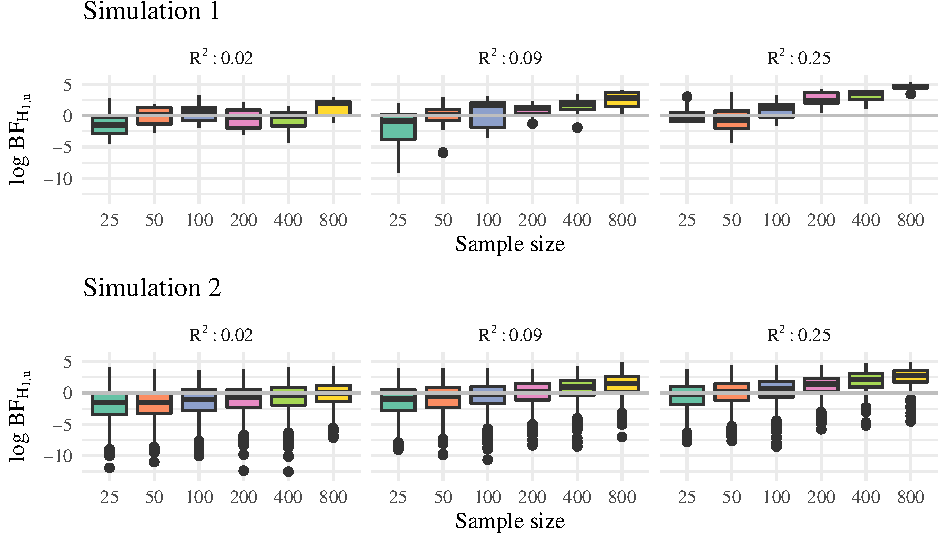
\includegraphics[width=1\linewidth]{manuscript_volker_files/figure-latex/BF12-1} \caption{Aggregated Bayes factors for hypothesis $H_{1,2}: \beta_4 < \beta_5 < \beta_6$ versus $H_u$ over three studies (with linear, logistic and probit models). In simulation 2, one of the three studies is randomly selected to have a small sample size ($n = 25$).}\label{fig:BF12}
\end{figure}

\begin{figure}
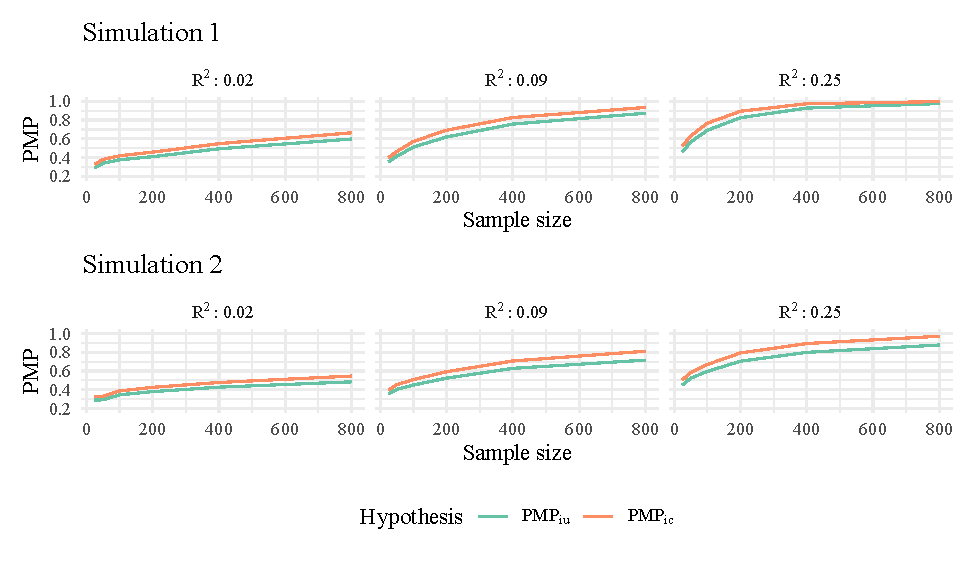
\includegraphics[width=1\linewidth]{manuscript_volker_files/figure-latex/PMP12-1} \caption{Aggregated $PMP$s for hypothesis $H_{1,2}: \beta_4 < \beta_5 < \beta_6$ versus $H_u$ or $H_c$ over three studies (with linear, logistic and probit models). In simulation 2, one of the three studies is randomly selected to have a small sample size ($n = 25$).}\label{fig:PMP12}
\end{figure}

In simulation 1 and 2, the aggregated Bayes factors for the true hypothesis \(H_{1,2}: \beta_4 < \beta_5 < \beta_6\) against the unconstrained hypothesis \(H_u\) increase with sample size and effect size (Figure \ref{fig:BF12}).
In simulation 1, for a small effect size (\(R^2 = 0.02\)), \(H_{1,2}\) is more often supported than \(H_u\) only when the sample size is at least \(n \geq 400\).
For \(n = 400\) and \(R^2 = 0.02\), the median aggregated Bayes factor (the middle horizontal black line in the box) is slightly above zero on the logarithmic scale, indicating that there is more support for the true hypothesis \(H_{1,2}\) than for \(H_u\) in slightly more than \(50\%\) of the iterations.
When the effect sizes increase, \(H_{1,2}\) is preferred over \(H_u\) in most iterations when \(n \geq 100\) or when \(n \geq 50\), for \(R^2 = 0.09\) and \(R^2 = 0.25\), respectively.
Note that evaluating a hypothesis against an unconstrained alternative yields a Bayes factor with an upper bound.
When the hypothesis fits the data perfectly (i.e., \(f_i = 1\)), the Bayes factor within a study cannot exceed \(1/c_i\).
Hence, the aggregated Bayes factor for three studies also has an upper bound.
For \(800\) observations per study and a large effect, the aggregated Bayes factor consistently approaches this upper bound.
In simulation 2, this upper bound is not reached in any condition, as the support for \(H_{1,2}\) is generally smaller than in simulation 1.
Likewise, larger sample sizes and effect sizes are required before \(H_{1,2}\) obtains more support than \(H_u\) in the majority of the iterations.
These findings are to be expected, because studies with the smallest sample size often provide support against \(H_{1,2}\).
Replacing a study with a larger sample size by a study with a sample size of \(n = 25\) thus leads to a decrease in the aggregated support.

Additionally, the aggregated support for the true hypothesis \(H_{1,2}\) versus both the unconstrained and complement hypothesis is quantified with posterior model probabilities (\(PMP\)s; Figure \ref{fig:PMP12}).
These results also show that the support for the true hypothesis increases with the sample and effect size.
For the smallest effect size, the average aggregated support does not exceed \(0.70\), indicating that \(H_{1,2}\) is hardly favored over \(H_u\).
For medium and large effects, the \(PMP\)s tend to \(1\) when the sample size is large enough.
Comparing simulation 1 and 2 shows that considering a single underpowered study in the set of studies substantially reduces the average aggregated \(PMP\)s.
When the effect size equals \(R^2 = 0.09\), the average aggregated support is larger for three studies with a sample size of \(n = 400\) (in simulation 1) than for two studies with a sample size of \(n = 800\) and one study with \(n = 25\) (in simulation 2).
Hence, although the total number of observations is higher in the latter setting, the average support for the true hypothesis is not, regardless of the alternative hypothesis.
Lastly, Figure \ref{fig:PMP12} shows that evaluating against the complement hypothesis consistently renders more support for the true hypothesis, although the difference is relatively small.

\hypertarget{simulation-3-and-4}{%
\subsubsection{Simulation 3 and 4}\label{simulation-3-and-4}}

\begin{figure}
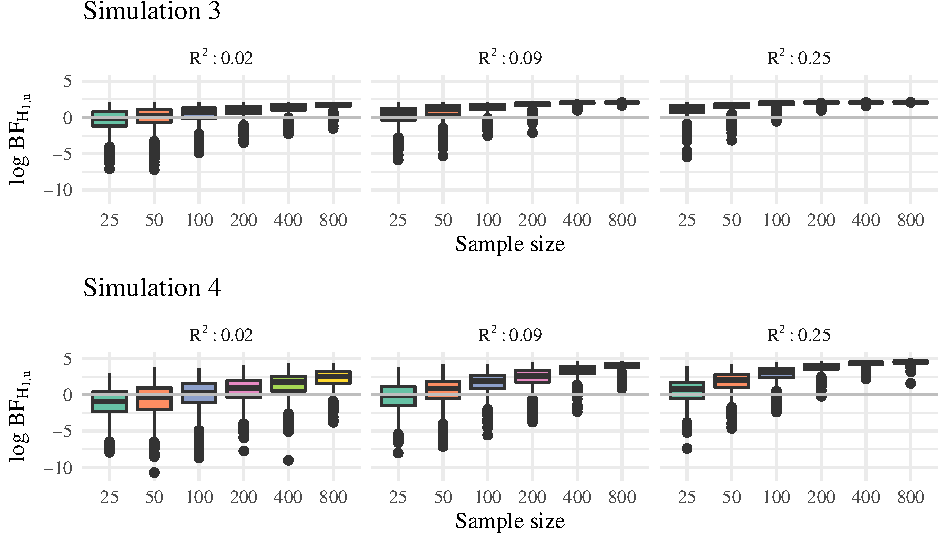
\includegraphics[width=1\linewidth]{manuscript_volker_files/figure-latex/BF34-1} \caption{Aggregated Bayes factors for hypothesis $H_3: \beta_6 > 0$ versus $H_u$ in simulation 3 and $H_4: \beta_{\text{low}} < \beta_{\text{medium}} < \beta_{\text{high}}$ versus $H_u$ in simulation 4 over three studies (with linear, logistic and probit models).}\label{fig:BF34}
\end{figure}

\begin{figure}
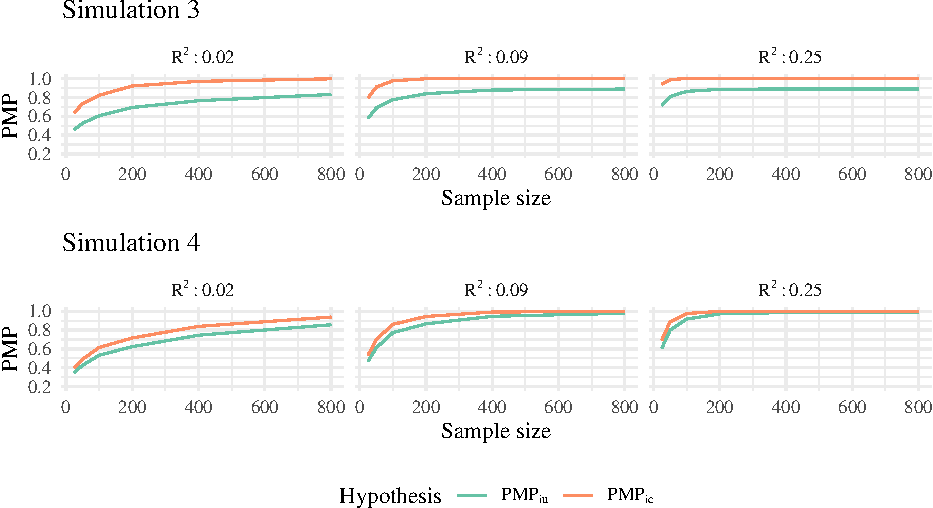
\includegraphics[width=1\linewidth]{manuscript_volker_files/figure-latex/PMP34-1} \caption{Aggregated $PMP$s for hypothesis $H_3: \beta_6 > 0$ versus $H_u$ and $H_c$ in simulation 3, and for $H_4: \beta_{\text{low}} < \beta_{\text{medium}} < \beta_{\text{high}}$ versus $H_u$ or $H_c$ in simulation 4 over three studies (with linear, logistic and probit models).}\label{fig:PMP34}
\end{figure}

Simulations 3 and 4 assess how the complexities of hypotheses affect \emph{BES}, by varying the operationalizations of a construct of interest.
Both simulations consider the expectation that \(X_6\) and \(Y\) are positively related (after controlling for \(X_1\) to \(X_5\)).
In simulation 3, \(X_6\) is considered as is, and the hypothesis \(H_3: \beta_6 > 0\) is evaluated.
In simulation 4, \(X_6\) is categorized into equally sized tertiles in each study, corresponding to \emph{low}, \emph{medium} and \emph{high} scoring groups \citep[which is, despite advice against it, a common procedure in many areas of research; e.g.,][]{bennette_against_2012, decoster_best_2011}.
Capturing the expected positive relationship between \(X_6\) and \(Y\) into an informative hypothesis yields \(H_4: \beta_{\text{low}} < \beta_{\text{medium}} < \beta_{\text{high}}\), where each coefficient reflects the mean of that group controlled for the 5 other variables.
Consequently, the complexity of \(H_4\) is substantially smaller than the complexity of \(H_3\), because more constraints are placed on the parameters.
Note, however, that categorizing a continuous variable also reduces the information in this variable, resulting in less statistical power.

Both Figure \ref{fig:BF34} and Figure \ref{fig:PMP34} show that the support for the true hypotheses \(H_3:\beta_6>0\) and \(H_4: \beta_{\text{low}} < \beta_{\text{medium}} < \beta_{\text{high}}\) increases with sample and effect size.
This is a recurrent pattern when the hypothesis of interest is in line with the specifications of the parameters.
In simulation 3, \(H_3\) obtains more support than \(H_u\) in more than \(50\%\) of the iterations when the sample size is at least \(n \geq 50\) for small effect sizes.
When medium and large effect sizes are considered, all sample sizes yield more support for \(H_3\) than \(H_u\) in the majority of the iterations.
For all effect sizes, the aggregated Bayes factor tends to its maximum if the sample size is large enough (given a complexity of \(c_i = 1/2\) per study in this simulation, the maximum aggregated Bayes factor is approximately equal to \(2.08\) on a logarithmic scale).
In contrast to simulation 3, there is in simulation 4 initially more support for \(H_u\) than for the hypothesis of interest for the smallest effect size.
Additionally, the true hypothesis \(H_4\) obtains less support than \(H_3\) in simulation 3 for the smallest sample sizes considered (i.e., for \(n \leq 100\) when \(R^2 = 0.02\), \(n \leq 50\) when \(R^2 = 0.09\) and for \(n = 25\) when \(R^2 = 0.25\)).
Both findings result from \(H_4\) having a smaller complexity than \(H_3\), which requires more statistical power to find support.
Yet, categorizing \(X_6\) results in less statistical power.
Whereas the aggregated support for \(H_3\) quickly reaches its maximum, the support for \(H_4\) continues to increase to higher levels.
For \(n = 800\) when \(R^2 = 0.09\), and for \(n \geq 400\) when \(R^2 = 0.25\), the support for \(H_4\) also reaches its maximum, but this maximum is substantially higher than the maximum in simulation 3, because the complexity of the hypothesis is smaller than in simulation 3.

The posterior model probabilities also clearly pinpoint the upper bound of the support for \(H_3\) when evaluated against \(H_u\) (Figure \ref{fig:PMP34}), especially for medium and large effects.
When \(H_3\) obtains full support from the data, the posterior model probabilities cannot exceed \(8/9\).
The support against the complement hypothesis is unrestricted, and therefore the support for \(H_3\) quickly tends to \(1\) for all effect sizes when compared to the complement hypothesis.
In simulation 4, the complexity of hypothesis \(H_4\) is relatively small.
Compared to simulation 3, the aggregated support for the more complex hypothesis \(H_4\) evaluated against \(H_u\) is therefore smaller for small sample sizes, but continues to increase to almost 1 when the support for \(H_3\) reaches its upper bound.
Additionally, there is only a small difference between evaluating \(H_4\) against the unconstrained and the complement hypothesis: the support for \(H_4\) is unconvincing initially, but increases with the sample and effect size for both alternatives.

\hypertarget{simulation-5-and-6}{%
\subsubsection{Simulation 5 and 6}\label{simulation-5-and-6}}

Simulations 5 and 6 also examine how evaluating hypotheses with different complexities affects \emph{BES} by varying the operationalizations of key constructs.
Assume that the variables \(X_2\), \(X_3\) and \(X_4\) are indicators of the same theoretical construct.
In simulation 5, the three indicators are collapsed into a single scale variable \(X_{\text{scale}}\) by taking the average of these variables for each observation in each of the studies, which is common scientific practice \citep{bauer_discrepancy_2016}.
Accordingly, the hypothesis under evaluation is \(H_5: \beta_{\text{scale}} > 0\), analysed in a model including an intercept and \(X_1\), \(X_5\) and \(X_6\) as control variables.
In simulation 6, the variables are left as is and included separately in the analyses, such that hypothesis \(H_6: \{\beta_2,\beta_3,\beta_4\} > 0\) is evaluated (with the same control variables).
Due to these specifications, \(H_5\) has a larger complexity than \(H_6\), due to \(H_6\) addressing multiple parameters, while \(\beta_{\text{scale}}\) has a smaller standard error than each of the individual regression coefficients (\(\beta_2\), \(\beta_3\) or \(\beta_4\)), resulting in more power to detect an effect.

In simulation 5, \(H_5\) obtains more support than \(H_u\) in more than \(50\%\) of the iterations over all sample and effect sizes except for \(n = 25\) and \(R^2 = 0.02\).
Additionally, the aggregated support for \(H_5: \beta_{\text{scale}}>0\) reaches its maximum for medium (at \(n \geq 400\)) and large (at \(n \geq 100\)) effect sizes.
In simulation 6, where hypothesis \(H_6\) concerns the separate predictors, the pattern is rather different.
When the effect size is small, the unconstrained hypothesis obtains most support, unless the sample size is at least \(n = 400\).
For medium and large effect sizes, \(H_6\) obtains more support than \(H_u\) when \(n \geq 100\) and \(n \geq 50\), respectively, and the support tends to much higher levels than in simulation 5.

Figure \ref{fig:PMP56} for simulation 5 and 6 shows a similar pattern as Figure \ref{fig:PMP34} for simulation 3 and 4.
The support for \(H_5\) tends to its maximum when compared with \(H_u\), especially for a large effect, while comparing against the complement leads to \(PMP\)s close to \(1\).
In simulation 6, the complexity of the hypothesis of interest is smaller, and the difference between evaluating against \(H_u\) or \(H_c\) decreases on the scale of the \(PMP\)s.
For small sample and effect sizes, this renders small \(PMP\)s, to such an extent that \(H_u\) is preferred over \(H_6\) for the smallest sample and effect sizes.
Yet, the smaller complexity also yields that the maximum \(PMP\) when evaluating against \(H_u\) is larger in simulation 6 than in simulation 5.
If the sample and effect size are sufficiently large, the \(PMP\)s for \(H_6\) are close to \(1\), regardless of whether \(H_6\) is evaluated against \(H_u\) or \(H_c\).
These results show the importance of having adequately powered studies when evaluating a specific hypothesis, because only then the hypothesis obtains convincing support.

\begin{figure}
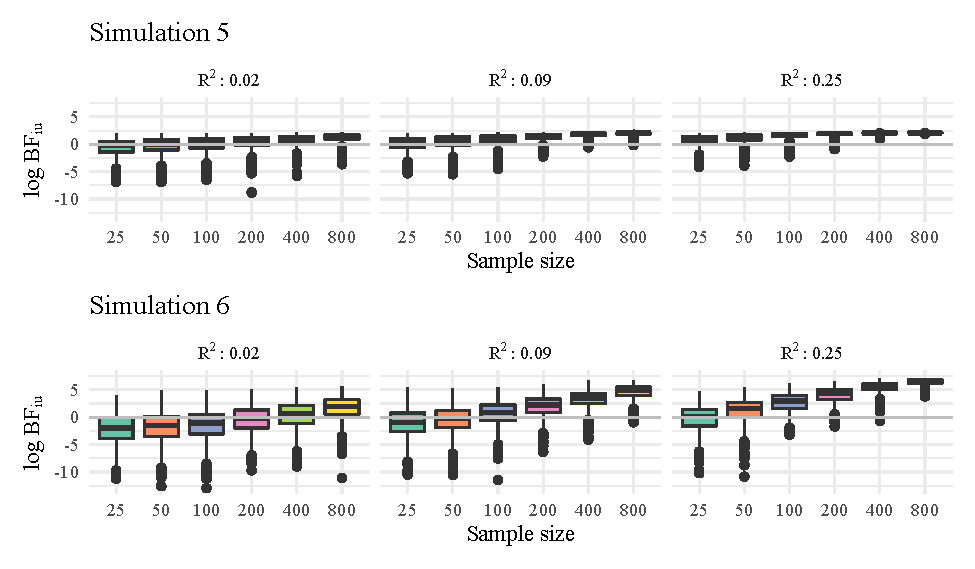
\includegraphics[width=1\linewidth]{manuscript_volker_files/figure-latex/BF56-1} \caption{Aggregated Bayes factors for hypothesis $H_5: \beta_{\text{scale}} > 0$ versus $H_u$ in simulation 5 and $H_6: \{\beta_2, \beta_3, \beta_4\} > 0$ versus $H_u$ in simulation 6 over three studies (with linear, logistic and probit models).}\label{fig:BF56}
\end{figure}

\begin{figure}
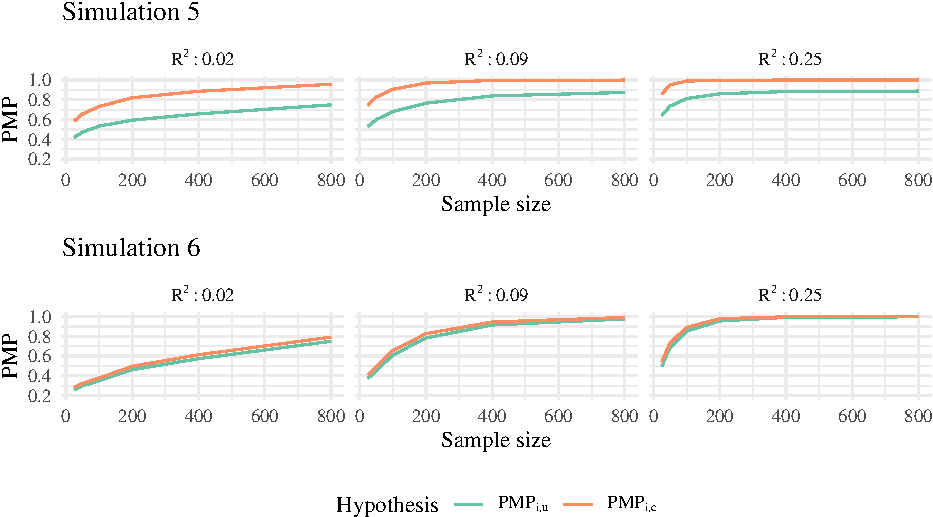
\includegraphics[width=1\linewidth]{manuscript_volker_files/figure-latex/PMP56-1} \caption{Aggregated $PMP$s for hypothesis $H_5: \beta_{\text{scale}} > 0$ versus $H_u$ and $H_c$ in simulation 5 and $H_6: \{\beta_2, \beta_3, \beta_4\} > 0$ versus $H_u$ or $H_c$ in simulation 6 over three studies (with linear, logistic and probit models).}\label{fig:PMP56}
\end{figure}

\hypertarget{simulation-7-and-8}{%
\subsubsection{Simulation 7 and 8}\label{simulation-7-and-8}}

\begin{figure}
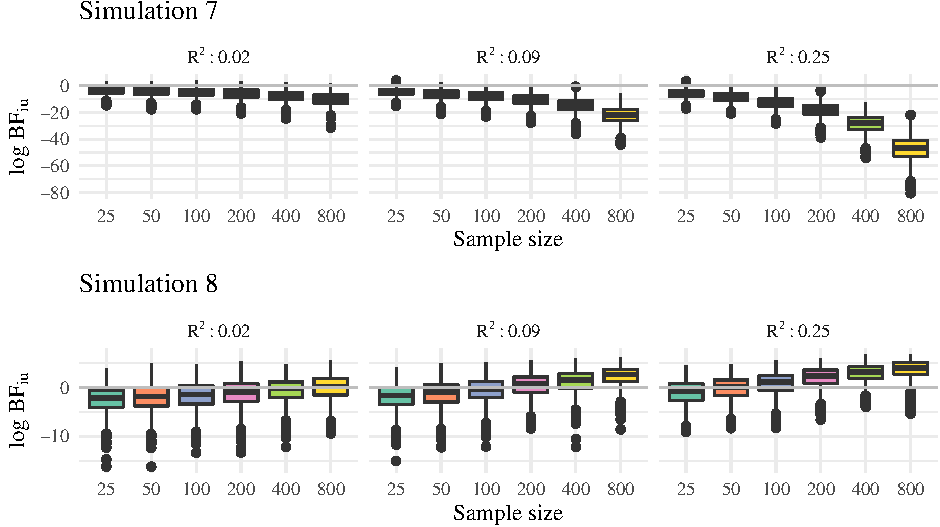
\includegraphics[width=1\linewidth]{manuscript_volker_files/figure-latex/BF78-1} \caption{Aggregated Bayes factors for the \textit{incorrect} hypothesis $H_7: \{\beta_2, \beta_3, \beta_4\} < 0$ versus $H_u$ in simulation 7 and \textit{partially incorrect} hypothesis $H_8: \{\beta_1, \beta_2, \beta_3\} > 0$ versus $H_u$ in simulation 8 over three studies (with linear, logistic and probit models). Note the different scaling of the y-axis.}\label{fig:BF78}
\end{figure}

\begin{figure}
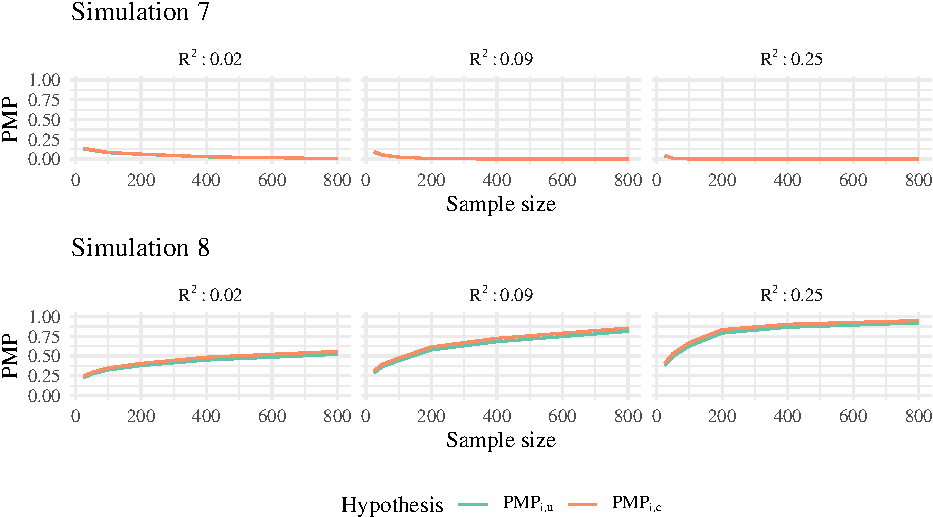
\includegraphics[width=1\linewidth]{manuscript_volker_files/figure-latex/PMP78-1} \caption{Aggregated $PMP$s for the \textit{incorrect} hypothesis $H_7: \{\beta_2, \beta_3, \beta_4\} < 0$ versus $H_u$ or $H_c$ in simulation 7 and $H_8: \{\beta_1, \beta_2, \beta_3\} > 0$ versus $H_u$ or $H_c$ in simulation 8 over three studies (with linear, logistic and probit models). Note that the line of $PMP_{i,u}$ in simulation 7 disappears because it is completely overlayed by the line for $PMP_{i,c}$.}\label{fig:PMP78}
\end{figure}

All previous simulations were concerned about whether \emph{BES} provides adequate results when a correct informative hypothesis is evaluated against the unconstrained or complement hypothesis.
In simulation 7 and 8, we assess the performance of \emph{BES} when the hypothesis of interest is incorrect.
We therefore expect \emph{BES} to render \emph{less} support for the hypotheses of interest when the sample and effect size increase.
In simulation 7, we consider \(H_7: \{\beta_2, \beta_3, \beta_4\} < 0\), implying a negative relationship between the indicators \(X_2\), \(X_3\) and \(X_4\) and the outcome \(Y\), which is for each parameter in the opposite direction as the true coefficient.
Hence, the unconstrained and complement alternative hypotheses are correct, although rather unspecific, in these simulations.
In simulation 8, we evaluate the \emph{partially incorrect} hypothesis \(H_8: \{\beta_1, \beta_2, \beta_3\} > 0\), which is correct for \(\beta_2\) and \(\beta_3\), but incorrect for \(\beta_1\), because \(\beta_1 = 0\).
This specification renders the unconstrained hypothesis correct, while the complement hypothesis is also partially incorrect, because the true parameter value of \(\beta_1\) is exactly on the boundary of \(H_8\) and \(H_c\).
In both simulations, the analysis model contains an intercept and the remaining variables as control variables.

Figure \ref{fig:BF78} shows that in simulation 7, the support for the incorrect hypothesis of interest quickly decreases, and renders more support for the unconstrained hypothesis.
In fact, already from the smallest sample sizes onward, there is less support for \(H_7\) than for the correct hypothesis \(H_u\), which further decreases when the sample and effect size increase.
In simulation 8, the support for the partially incorrect hypothesis \(H_8\) increases, rather than decreases, with the sample size and effect size (Figure \ref{fig:BF78}; note the different scale of the y-axis compared to simulation 7).
Whereas for small sample and effect sizes the correct unconstrained hypothesis is preferred over \(H_8\), the partially incorrect \(H_8\) eventually obtains more support.
Although this behavior is undesirable, it is not surprising.
The posterior distribution of \(\beta_1\) is, on average, for \(50\%\) in line with the constraints imposed by \(H_8\), because the true parameter value is on the boundary of the hypothesis, while for larger sample and effect sizes, the posterior of \(\beta_2\) and \(\beta_3\) is almost completely in line with this hypothesis.
Hence, even though the hypothesis is partially incorrect, the fit generally exceeds the complexity.

The posterior model probabilities in Figure \ref{fig:PMP78} tell a similar story.
The average aggregated \(PMP\)s for the incorrect \(H_7\) render very strong support against this hypothesis, for all sample sizes and effect sizes and for both alternative hypotheses (note that the line for \(H_u\) is almost completely covered by the line for \(H_c\)).
In simulation 8, the average aggregated \(PMP\)s are indecisive under a small effect size, but favor the partially incorrect hypothesis \(H_8\) over the correct unconstrained and partially incorrect complement hypothesis when the effect and sample size increase.
The difference between evaluating against \(H_u\) and \(H_c\) is negligible, although \(H_u\) is the only correct hypothesis in this simulation.

\hypertarget{discussion-simulations-part-1}{%
\subsubsection{Discussion simulations part 1}\label{discussion-simulations-part-1}}

The first simulations show that \emph{BES} performs adequately, in the sense that the aggregated support for correct hypotheses increases with the sample and effect size (simulations 1-6).
Moreover, simulation 7 shows that incorrect hypotheses obtain less support when the sample and effect size increase.
Hence, when the individual studies have sufficient power, \emph{BES} enables researchers to aggregate support for complex informative hypotheses over studies.
Yet, in simulation 8, \emph{BES} functions unsatisfactorily, because with increasing sample and effect sizes, it renders increasing support for the partially incorrect hypothesis.
Note, however, that this hypothesis is very close to the truth \citep[Bayes factors have been proven to prefer the model that is closest, in terms of Kullback-Leibler divergence, to the true data-generating model; see][]{ly_bf_2016, berger2013statistical}.
When evaluating inequality-constrained hypotheses against the unconstrained or complement alternative, support for incorrect hypotheses can only keep increasing with the sample and effect size when no parameters truly violate the hypothesis of interest (i.e, all parameters are on or within the boundary values of the hypothesis).
If at least one of the parameters falls outside the constraints imposed by the hypothesis, the fit will tend to zero for sufficiently large sample sizes.
Yet, the fact that partially incorrect hypotheses can obtain substantial support warrants that researchers not only assess the aggregated support, but also consider the results of the individual studies.
If some of the estimated parameters are typically in line with the hypothesis while others fluctuate around the hypothesized value between studies, further investigation is required, potentially leading to theoretical refinements, that should be evaluated with new data, regardless of the aggregated support.

The main focus of the previous simulations was on how the complexity of the hypotheses affects the performance of \emph{BES}.
Especially in the context of conceptual replications, researchers might want to aggregate the support for hypotheses with different complexities, due to different operationalizations or measurement instruments.
Unlike conventional research synthesis approaches, \emph{BES} allows to aggregate support for equivalent hypotheses with different complexities and, as simulations 3 to 6 show, renders correct results when the individual studies have sufficient power.
Hence, the support for an overarching theory over studies can be quantified with \emph{BES}, even when studies use different operationalizations.
Our findings may even insinuate that, under sufficient power, common procedures in data handling that result in hypotheses with smaller complexities, such as categorizing continuous variables or assessing individual indicators rather than scale scores, can lead to more support on the aggregate level.
After all, the hypotheses with the smallest complexities within a set of studies have the highest upper bound for the Bayes factor against the unconstrained hypothesis.
However, this conclusion should be drawn with caution, because it only holds when evaluating against the unconstrained, but not when evaluating against the complement hypothesis.
The Bayes factor against the complement tends to infinity when the data fits the hypothesis perfectly, and thus does not benefit from evaluating more specific hypotheses.

Similarly to previous work \citep[e.g.,][]{klugkist_volker}, our simulations confirm that if individual studies lack statistical power, \emph{BES} has difficulties with finding support for the correct hypothesis.
Specifically, including a single underpowered study, as in simulation 1 and 2, reduces the performance of \emph{BES}.
Moreover, aggregating over three adequately powered studies provides more support for the correct hypothesis than aggregating over two adequately powered studies and a single underpowered study, even if the total number of observations is higher in the latter scenario.
Whereas conventional approaches for research synthesis as meta-analysis or Bayesian sequential updating can overcome such power issues, \emph{BES} typically does not.
Unlike these approaches, \emph{BES} does not pool data or parameter estimates, but rather aggregates the support for the hypothesis of interest in each study.
Hence, some support against the hypothesis of interest in each study will accumulate when aggregating over studies.

Such power issues are amplified when the complexity of the hypothesis of interest decreases (see simulations 3 to 6).
With insufficient power, parameters may not be estimated accurately.
If a hypothesis places constraints on multiple parameters, the probability increases that at least one of the constraints is violated, which substantially reduces the fit of the hypothesis.
Common procedures in data handling that reduce the complexity of the hypothesis (e.g., categorizing continuous variables), and simultaneously the power of the analysis, may thus have adverse consequences for \emph{BES}.
Although our previous simulations show the vulnerability of \emph{BES} to power issues, substantial uncertainty remains about the extent to which these problems depend on (i) the number of studies included, (ii) the complexity of the hypothesis of interest, and (iii) the choice of alternative hypothesis.
Evaluating against the complement hypothesis yields a more powerful evaluation of the hypothesis of interest, which may reduce the severity of power issues.
Our findings also suggest that including more studies with insufficient power may lead to decreasing support for the correct hypothesis.
We address these questions in the subsequent section.

\hypertarget{simulations-part-2---power-issues-of-bes}{%
\subsection{\texorpdfstring{Simulations part 2 - power issues of \emph{BES}}{Simulations part 2 - power issues of BES}}\label{simulations-part-2---power-issues-of-bes}}

Part two of the simulations zooms in on the extent to which \emph{BES} renders support for \emph{correct} hypotheses as the number of studies increases, while comparing between studies with and without sufficient power.
Moreover, we further assess the influence of the complexity of the hypothesis and the choice of alternative hypothesis (i.e., an unconstrained or a complement alternative hypothesis) on the amount of aggregated support.
We consider the same data-generating mechanism as in previous simulations, but restrict the simulations to OLS regression for the sake of brevity (although other models yield equivalent results).
To keep the results tractable, only one effect size and two sample sizes are considered (\(R^2 = 0.09\) and \(n \in \{25, 200\}\)), representing underpowered and adequately powered studies, respectively.
The number of studies is varied from \(1\) to \(150\), and the number of iterations is again set to 1000.
In all three simulations in part two, the cumulative aggregated support is assessed for the hypotheses of interest against an unconstrained and a complement alternative hypothesis for the two sample sizes considered.

\hypertarget{simulations-9-10-and-11}{%
\subsubsection{Simulations 9, 10 and 11}\label{simulations-9-10-and-11}}

\begin{figure}[!t]
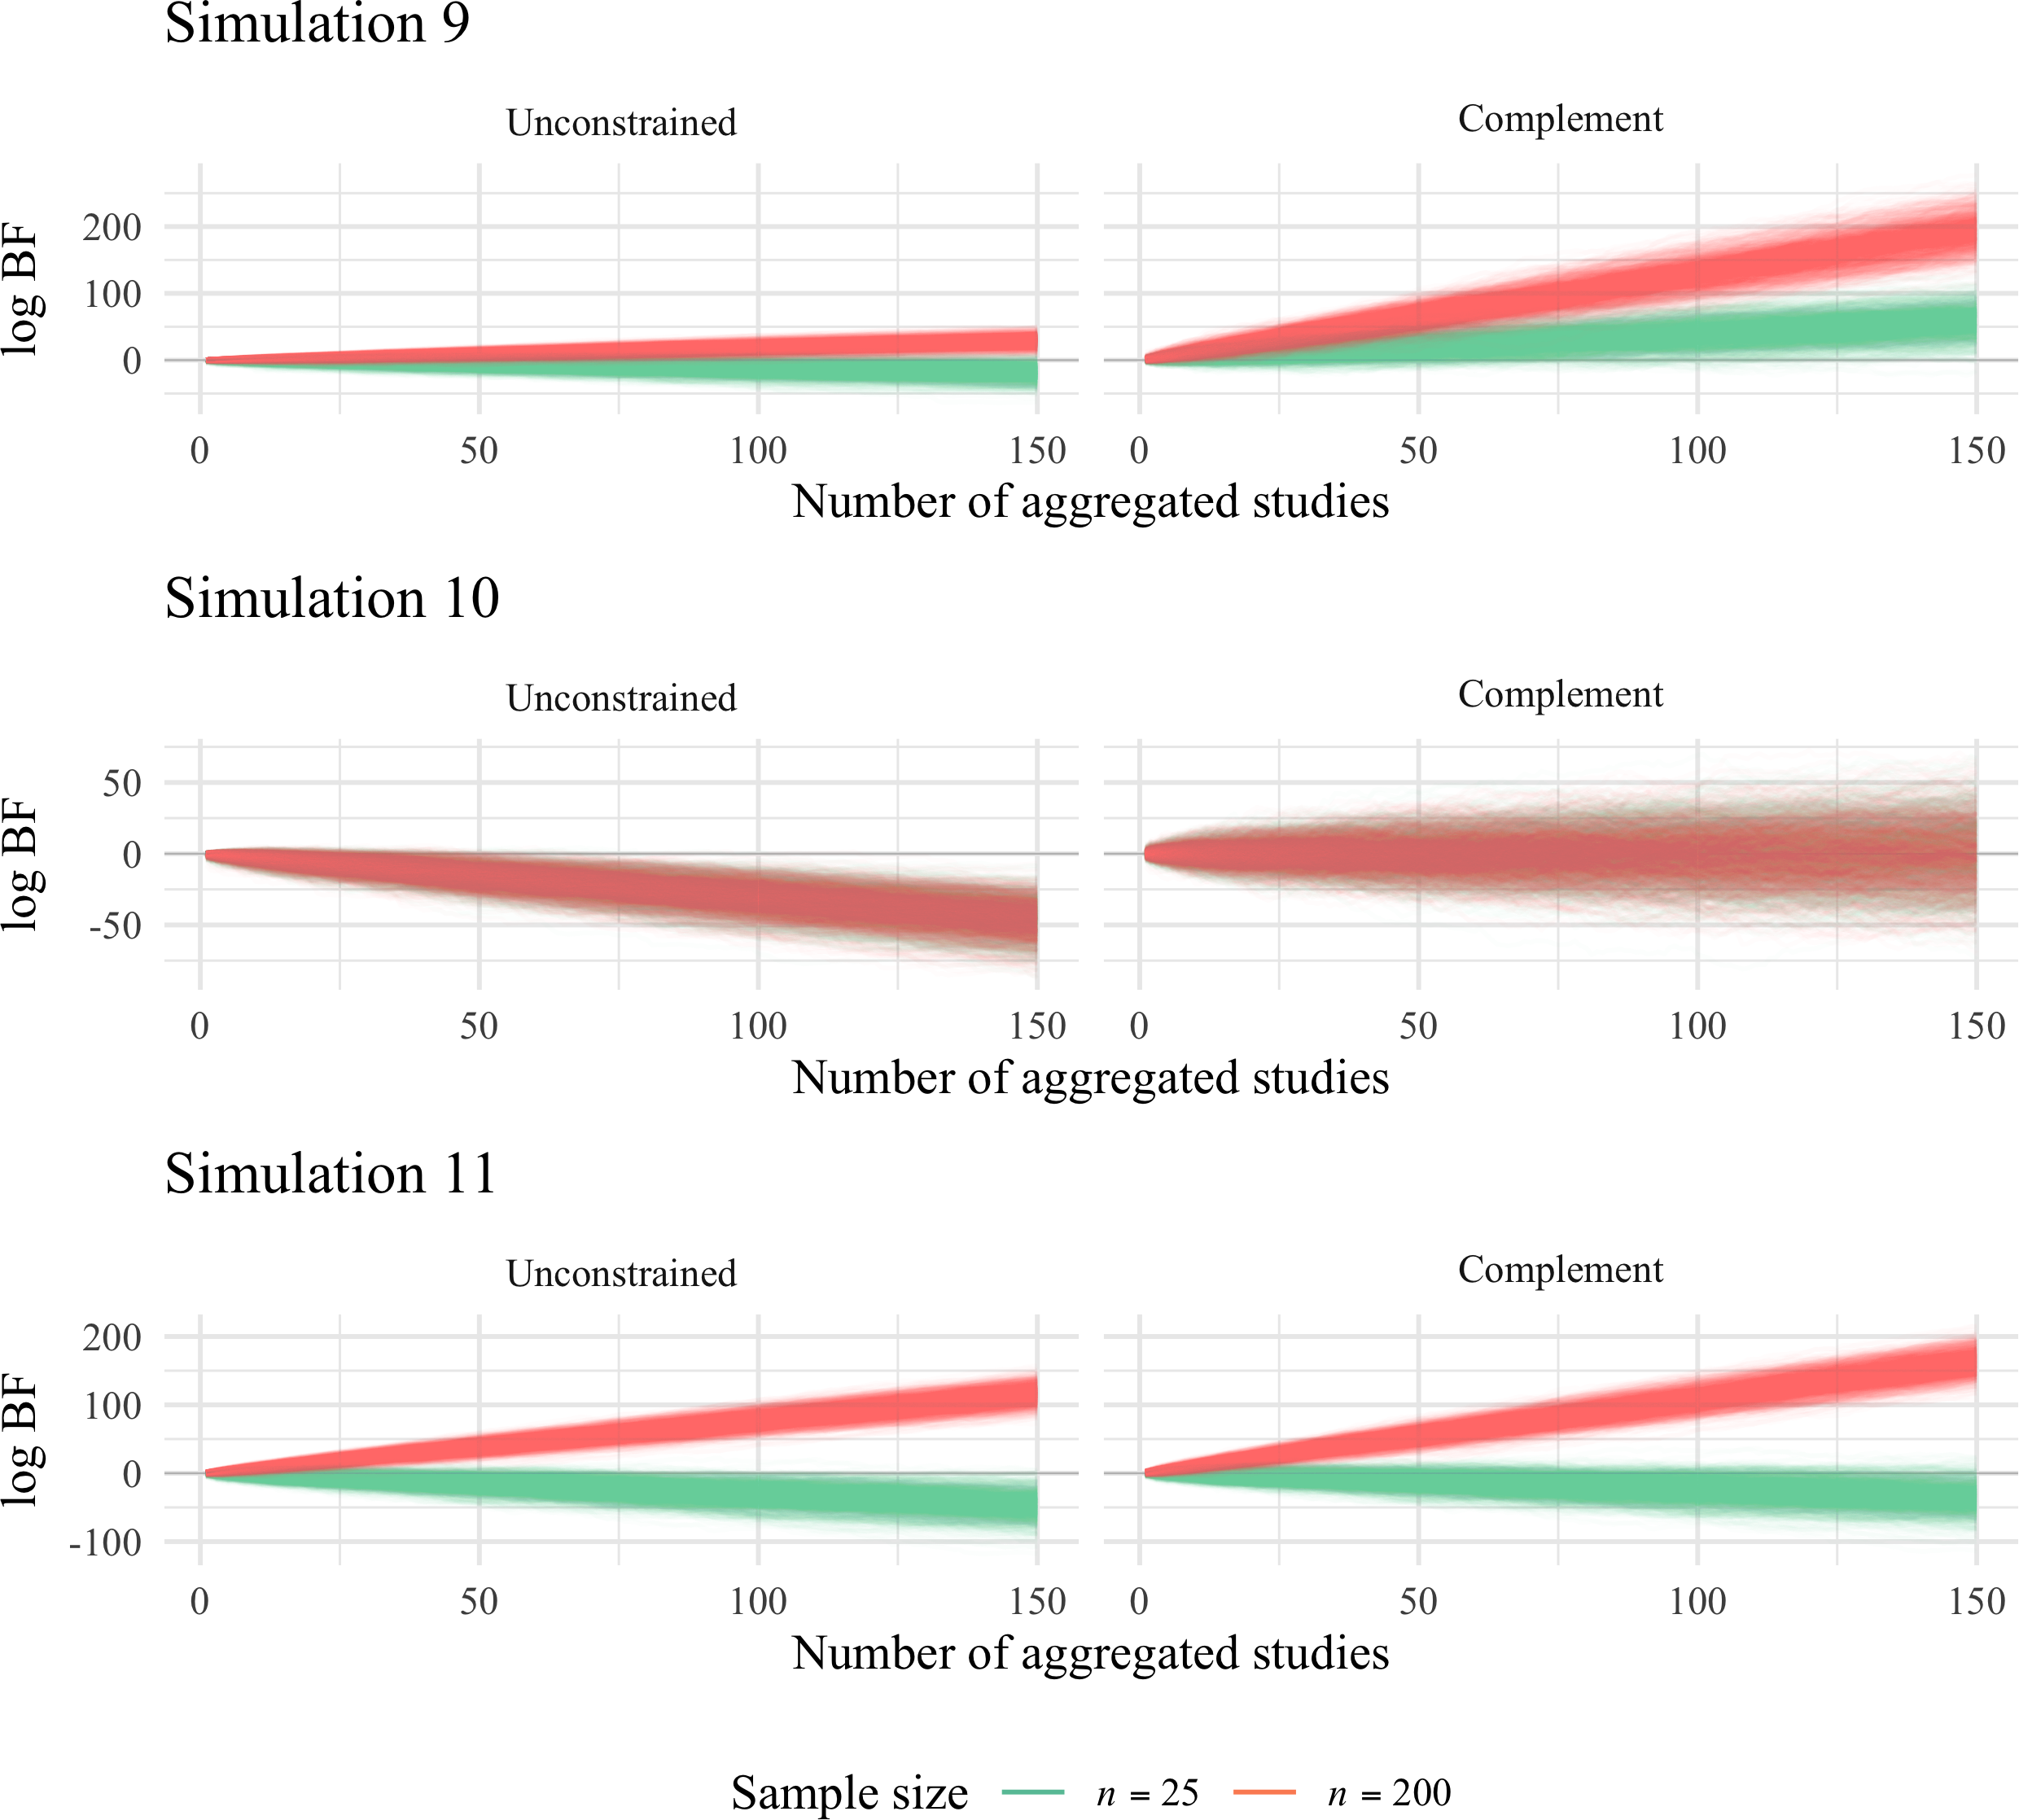
\includegraphics[width=1\linewidth]{manuscript_volker_files/figure-latex/BF91011-1} \caption{Cumulative aggregated Bayes factors for the correct hypothesis $H_9: \beta_2 > 0$ in simulation 9, $H_{10}: \beta_1 > 0$ in simulation 10 and $H_{11}: \{\beta_2, \beta_3, \beta_4\} > 0$ in simulation 11, versus an unconstrained and complement alternative hypothesis over 1 to 150 studies, based on OLS regression models. Note (i) that the scale of the y axis differs between the simulations, and (ii) that the lines for the two sample sizes are completely overlapping in simulation 10.}\label{fig:BF91011}
\end{figure}

In simulation 9, we evaluate \(H_9: \beta_2 > 0\) against the unconstrained and complement hypotheses and assess the influence of the alternative hypothesis for underpowered and adequately powered studies.
Recall that \(H_9\) is correct, as the population value of the coefficient equals \(\beta_2 = 0.054\) (Table \ref{tab:coefs}).
For studies with a small sample size, Figure \ref{fig:BF91011} shows that evaluating against \(H_u\) renders decreasing support for the correct hypothesis \(H_9\) when the number of studies increases.
After conducting \(150\) studies, \(H_u\) is clearly preferred over \(H_9\).
For larger samples (i.e., \(n = 200\)), the correct hypothesis \(H_9\) is consistently preferred over \(H_u\).
Evaluating \(H_9\) against the complement hypothesis consistently renders support for \(H_9\) for both sample sizes, although the support increases faster for larger samples.
Additionally, the absence of an upper bound yields that the support for \(H_9\) increases at a faster rate when evaluated against \(H_c\) than when evaluated against \(H_u\).

In simulation 10, we investigate a similar, but incorrect, hypothesis \(H_{10}: \beta_1 > 0\) (\(\beta_{1}=0\) in the population; Table \ref{tab:coefs}).
This renders \(H_u\) the only true hypothesis, because \(H_c\) and \(H_{10}\) are equally incorrect.
Evaluating against the unconstrained hypothesis consistently renders more support for \(H_u\) over \(H_{10}\), regardless of the sample size.
When the true parameter value is on the boundary of the hypothesis of interest, comparing against the complement renders substantial variability in the support for \(H_{10}\) and \(H_c\), regardless of the sample size (note that the lines for the two sample sizes are completely overlapping for simulation 10).
Although \(H_{10}\) and \(H_c\) obtain, on average, the same support, the individual iterations show considerable support for either of the two.
Hence, there is a downside to evaluating against the complement hypothesis, because it is possible to find considerable support for or against a hypothesis on the aggregate level, while there is no effect in reality.

Simulation 11 evaluates the \emph{correct} \(H_{11}: \{\beta_2, \beta_3, \beta_4\} > 0\) (\(\beta_2 = \beta_3 = \beta_4 = 0.054\) in the population; Table \ref{tab:coefs}), which is the same hypothesis as evaluated in simulation 6.
Whereas the hypotheses of interest in simulations 9 and 10 were balanced with their respective complements, in the sense that both have a complexity of \(c_i = 1/2\), \(H_{11}\) is not.
Simulation 11 in Figure \ref{fig:BF91011} shows that the support for the correct hypothesis \(H_{11}\) decreases when more small sample studies are included, regardless of the alternative hypothesis, although there is somewhat more support on average when evaluating against the complement.
Hence, when the complexity of the hypothesis of interest and its complement are not balanced, the aggregated Bayes factor does not necessarily tend to the \emph{correct} hypothesis, but favors the more general alternatives.
When the sample size is sufficiently large, the issue dissolves, and the support for \(H_{11}\) increases substantially when more studies are added, for both alternative hypotheses.

Informative hypotheses on multiple parameters can be separated in multiple, simpler hypotheses.
For example, the hypothesis \(H_{11}\) can be deconstructed into three simpler hypotheses (\(H_{11_a}: \beta_2 > 0\), \(H_{11_b}: \beta_3 > 0\) and \(H_{11_c}: \beta_4 > 0\)).
Accordingly, each component is balanced with its complement.
Evaluating each sub-hypothesis against the unconstrained hypothesis and its complements yields an identical outcome as in simulation 9.
Hence, evaluating against the unconstrained hypotheses renders support for each sub-hypothesis when the sample size is large, but favors \(H_u\) when the sample size is small.
When evaluating each hypothesis against its complement, the sub-hypotheses obtain considerable support, regardless of the sample size.
Hence, whereas evaluating a multifaceted hypothesis as \(H_{11}\) leads to support against the hypothesis of interest, evaluating the separate components of this hypothesis provides support for each component.

\hypertarget{discussion-simulation-part-2}{%
\subsubsection{Discussion simulation part 2}\label{discussion-simulation-part-2}}

Part two of the simulations further assessed the sensitivity of \emph{BES} to power issues.
When the studies are adequately powered, the support for the true hypothesis is consistently found over the situations.
However, when evaluating a correct hypothesis on a single regression parameter in studies that lack statistical power, the aggregated support for the unconstrained hypothesis increases with the number of studies.
If the hypothesis of interest is balanced with its complement, such that both have the same complexity,
evaluating against the complement hypothesis is not sensitive to the power within the studies.
This difference is due to the fact that evaluating against the unconstrained hypothesis weighs evidence against the hypothesis of interest heavier than evidence for this hypothesis.
That is, the Bayes factor for a hypothesis evaluated against the unconstrained has an upper bound, while the lower bound of \(0\) corresponds to infinite support for the unconstrained.
Note that when studies have little power, parameter estimates vary considerably.
If a single study finds, by chance, substantial support against the hypothesis of interest (e.g., a fit of \(f_i=0.1\) and a complexity of \(c_i=0.5\), rendering a Bayes factor of \(BF_{iu}=0.2\)), adding two new studies that perfectly fit the hypothesis of interest (resulting in a Bayes factor of \(BF_{iu}=1/0.5=2\) per study) yields an aggregate Bayes factor of \(BF^T_{iu}=0.8\).
On the aggregate level, there thus is still more support for the unconstrained hypothesis.
Evaluating against the complement weighs the evidence for both hypotheses equally heavy under these circumstances, and thus provides increasing support for the correct hypothesis.

When the hypothesis of interest places constraints on multiple parameters, evaluating against the complement results in somewhat more power than evaluating against the unconstrained, but both provide support against the correct hypothesis of interest when the studies are underpowered.
Whereas part one of the simulations already showed that evaluating specific hypotheses is only feasible when studies are adequately powered, part two of the simulations shows that adding more studies provides no solution.
The hypothesis of interest constrained three parameters, resulting in 8 possible parameter orderings of which only one was correct.
When the individual studies have little power, the probability that at least one of the estimated parameters falls outside the constraints imposed by the hypothesis is considerable, due to the fact that the parameters are generally estimated inaccurately.
Regardless of which constraint is violated, the hypothesis may fit poorly in each study, resulting in aggregated support against the hypothesis that further increases with the number of studies.
This issue can be remedied by deconstructing the hypothesis space in smaller regions, and evaluating each part separately against each complement.
This approach has two advantages.
First, less statistical power is required to find support for the correct hypothesis.
Especially, if each sub-hypothesis is balanced with its complement, \emph{BES} will provide support for the correct hypothesis if enough studies are included.
Second, this approach allows to evaluate whether each component of the hypothesis obtains support after aggregation.
If the overall hypothesis is incorrect, evaluating the sub-hypotheses highlights which parts of the overall hypothesis are not supported.
In this sense, deconstructing the hypothesis space can help to further refine the theory.

Although evaluating hypotheses against their balanced complements has advantages, it is no panacea.
Simulation 10 shows that if the true parameter value is on the boundary of the hypothesis of interest and its complement, it is possible to find overwhelming support for either of the two.
The implications hereof reach beyond \emph{BES}, because already within individual studies strong support can be obtained for incorrect hypotheses.
\emph{BES} further amplifies this problem.
The variability of the aggregated support increases with the number of studies, such that overwhelming support for one of the two hypotheses regularly occurs.
This problem can be dealt with in three ways.
First, one could consider an equality-constrained hypothesis (e.g., \(H_i: \beta_1=0\)).
In contrast to evaluating inequality-constrained hypotheses \citep{klugkist_bf_2007}, however, evaluating equality-constrained hypotheses with a Bayes factor is sensitive to the scale (i.e., variance) of the prior distribution within a study \citep{hoijtink_prior_2021, tendeiro_kiers_2019}.
Accordingly, a sensitivity analysis of the Bayes factor within a study is generally required \citep{hoijtink_prior_2021}, which induces uncertainty regarding the ``correct'' Bayes factor within a study, let alone when aggregated over studies.
Additionally, Bayes factors on equality-constrained hypotheses versus unconstrained alternatives tend to provide overly strong evidence in favor of the former, especially when the power of the study is relatively small \citep[e.g.,][]{tendeiro_kiers_2019}.
This approach might induce more severe power issues when using \emph{BES}.
Future research should address these considerations in more detail.
Second, one could evaluate a hypothesis with a boundary on the minimum relevant effect size versus its complement.
Then, if support for the hypothesis is found, one can be sure that there is an effect that is relevant.
If no support is found, either there is no effect, or the effect is too small to be relevant.
Third, the hypothesis of interest can be evaluated against both the unconstrained and the complement hypothesis.
If both render support for (or against) the hypothesis of interest, one can conclude that this hypothesis provides an accurate description of the data.
If the results are contradictory, researchers may have to acknowledge that considerable uncertainty remains, and that more (adequately powered) studies on the topic are required for a robust conclusion.

\hypertarget{conclusion}{%
\section{Conclusion}\label{conclusion}}

In multiple simulations, we examined the performance of Bayesian Evidence Synthesis when evaluating hypotheses with different complexities against different alternatives under various sample and effect sizes.
Part one of the simulations showed that \emph{BES} is applicable regardless of differences in analysis models in the set of studies under consideration, and renders correct results if the individual studies have sufficient statistical power.
The simulations emphasized the importance of power when aggregating evidence over studies, especially when evaluating more specific hypotheses.
For small sample and effect sizes, evaluating a hypothesis with a relatively small complexity generally results in support for the unconstrained and complement hypotheses.
If the aggregated Bayes factors within the studies yield more support for the alternatives than for the specific correct hypothesis, adding more studies that are also underpowered will not solve the issue.
In this sense, \emph{BES} clearly differs from conventional methods for research synthesis (e.g., (Bayesian) meta-analysis and Bayesian sequential updating).
Whereas the former two approaches increase the statistical power when incorporating evidence from additional studies, \emph{BES}, in general, does not.

Part two of the simulations underscored that adding more underpowered studies only amplifies the issue.
Aggregating the evidence for a hypothesis with a small complexity consistently renders support against this hypothesis when the studies lack power, regardless of the alternative hypothesis.
If the hypothesis of interest and its complement are balanced, however, the aggregated Bayes factor will eventually show support for the correct hypothesis, if either the hypothesis of interest or its complement is correct.
As a consequence, it can be worthwhile to separate a specific hypothesis with multiple parameter constraints into multiple sub-hypotheses that are all balanced with their complements.
If either the sub-hypothesis or its complement is correct, the aggregated Bayes factor will provide support for the correct hypothesis.
Moreover, evaluating sub-hypotheses allows to assess which constraints imposed by the overall hypothesis are supported by the data and which are not, providing a more detailed overview of the support in the studies for the overarching hypothesis.

Overall, evaluating against the complement has advantages over evaluating against the unconstrained.
Evaluating against the complement results in more statistical power, and the resulting Bayes factor has no upper bound.
Moreover, in a practical research setting, some studies may have insufficient power, while others have sufficient power.
In such instances, adequately powered studies will eventually provide decisive support when evaluated against the complement hypothesis.
Yet, when evaluating against the unconstrained, the underpowered studies may jeopardize the aggregated evidence.
That is, if underpowered studies occasionally render support against the hypothesis of interest, the adequately powered studies may not be able to compensate because of the upper bound.
A disadvantage of evaluating against the complement occurs if the true parameter value is on the boundary of the hypothesis of interest and its complement, because the aggregated support becomes highly variable.
We discussed several approaches to deal with this issue, but future research should compare the advantages and disadvantages of these approaches.

Lastly, \emph{BES} has strengths that conventional methods for research synthesis lack, in the sense that \emph{BES} is capable of aggregating the support for hypotheses over studies with different designs (i.e., experimental, cross-sectional or longitudinal) or different methodologies.
However, there are situations in which solely evaluating the aggregated evidence can fall short, for example when the hypothesis of interest is too specific for the statistical power of a study, or when the hypothesis under evaluation is partially incorrect.
Hence, researchers should not only blindly follow the results after aggregation, but also assess the results in the individual studies.
The results on the level of the individual studies may give an additional sense of the robustness of the results over different situations, while simultaneously signifying potential moderating circumstances of the effect of interest.
Such additional information might raise doubts about the robustness of the conclusions in specific scenarios, but can also hint towards interesting new areas of research or corroborate the conclusions from the synthesis.
Overall, \emph{BES} provides great opportunities to aggregate scientific evidence over heterogeneous studies, but solely relying on this aggregate derogates from the wealth of information in the individual studies.

\bibliography{thesis.bib}


\end{document}
